% Options for packages loaded elsewhere
\PassOptionsToPackage{unicode}{hyperref}
\PassOptionsToPackage{hyphens}{url}
%
\documentclass[
]{book}
\usepackage{amsmath,amssymb}
\usepackage{iftex}
\ifPDFTeX
  \usepackage[T1]{fontenc}
  \usepackage[utf8]{inputenc}
  \usepackage{textcomp} % provide euro and other symbols
\else % if luatex or xetex
  \usepackage{unicode-math} % this also loads fontspec
  \defaultfontfeatures{Scale=MatchLowercase}
  \defaultfontfeatures[\rmfamily]{Ligatures=TeX,Scale=1}
\fi
\usepackage{lmodern}
\ifPDFTeX\else
  % xetex/luatex font selection
\fi
% Use upquote if available, for straight quotes in verbatim environments
\IfFileExists{upquote.sty}{\usepackage{upquote}}{}
\IfFileExists{microtype.sty}{% use microtype if available
  \usepackage[]{microtype}
  \UseMicrotypeSet[protrusion]{basicmath} % disable protrusion for tt fonts
}{}
\makeatletter
\@ifundefined{KOMAClassName}{% if non-KOMA class
  \IfFileExists{parskip.sty}{%
    \usepackage{parskip}
  }{% else
    \setlength{\parindent}{0pt}
    \setlength{\parskip}{6pt plus 2pt minus 1pt}}
}{% if KOMA class
  \KOMAoptions{parskip=half}}
\makeatother
\usepackage{xcolor}
\usepackage{color}
\usepackage{fancyvrb}
\newcommand{\VerbBar}{|}
\newcommand{\VERB}{\Verb[commandchars=\\\{\}]}
\DefineVerbatimEnvironment{Highlighting}{Verbatim}{commandchars=\\\{\}}
% Add ',fontsize=\small' for more characters per line
\usepackage{framed}
\definecolor{shadecolor}{RGB}{248,248,248}
\newenvironment{Shaded}{\begin{snugshade}}{\end{snugshade}}
\newcommand{\AlertTok}[1]{\textcolor[rgb]{0.94,0.16,0.16}{#1}}
\newcommand{\AnnotationTok}[1]{\textcolor[rgb]{0.56,0.35,0.01}{\textbf{\textit{#1}}}}
\newcommand{\AttributeTok}[1]{\textcolor[rgb]{0.13,0.29,0.53}{#1}}
\newcommand{\BaseNTok}[1]{\textcolor[rgb]{0.00,0.00,0.81}{#1}}
\newcommand{\BuiltInTok}[1]{#1}
\newcommand{\CharTok}[1]{\textcolor[rgb]{0.31,0.60,0.02}{#1}}
\newcommand{\CommentTok}[1]{\textcolor[rgb]{0.56,0.35,0.01}{\textit{#1}}}
\newcommand{\CommentVarTok}[1]{\textcolor[rgb]{0.56,0.35,0.01}{\textbf{\textit{#1}}}}
\newcommand{\ConstantTok}[1]{\textcolor[rgb]{0.56,0.35,0.01}{#1}}
\newcommand{\ControlFlowTok}[1]{\textcolor[rgb]{0.13,0.29,0.53}{\textbf{#1}}}
\newcommand{\DataTypeTok}[1]{\textcolor[rgb]{0.13,0.29,0.53}{#1}}
\newcommand{\DecValTok}[1]{\textcolor[rgb]{0.00,0.00,0.81}{#1}}
\newcommand{\DocumentationTok}[1]{\textcolor[rgb]{0.56,0.35,0.01}{\textbf{\textit{#1}}}}
\newcommand{\ErrorTok}[1]{\textcolor[rgb]{0.64,0.00,0.00}{\textbf{#1}}}
\newcommand{\ExtensionTok}[1]{#1}
\newcommand{\FloatTok}[1]{\textcolor[rgb]{0.00,0.00,0.81}{#1}}
\newcommand{\FunctionTok}[1]{\textcolor[rgb]{0.13,0.29,0.53}{\textbf{#1}}}
\newcommand{\ImportTok}[1]{#1}
\newcommand{\InformationTok}[1]{\textcolor[rgb]{0.56,0.35,0.01}{\textbf{\textit{#1}}}}
\newcommand{\KeywordTok}[1]{\textcolor[rgb]{0.13,0.29,0.53}{\textbf{#1}}}
\newcommand{\NormalTok}[1]{#1}
\newcommand{\OperatorTok}[1]{\textcolor[rgb]{0.81,0.36,0.00}{\textbf{#1}}}
\newcommand{\OtherTok}[1]{\textcolor[rgb]{0.56,0.35,0.01}{#1}}
\newcommand{\PreprocessorTok}[1]{\textcolor[rgb]{0.56,0.35,0.01}{\textit{#1}}}
\newcommand{\RegionMarkerTok}[1]{#1}
\newcommand{\SpecialCharTok}[1]{\textcolor[rgb]{0.81,0.36,0.00}{\textbf{#1}}}
\newcommand{\SpecialStringTok}[1]{\textcolor[rgb]{0.31,0.60,0.02}{#1}}
\newcommand{\StringTok}[1]{\textcolor[rgb]{0.31,0.60,0.02}{#1}}
\newcommand{\VariableTok}[1]{\textcolor[rgb]{0.00,0.00,0.00}{#1}}
\newcommand{\VerbatimStringTok}[1]{\textcolor[rgb]{0.31,0.60,0.02}{#1}}
\newcommand{\WarningTok}[1]{\textcolor[rgb]{0.56,0.35,0.01}{\textbf{\textit{#1}}}}
\usepackage{longtable,booktabs,array}
\usepackage{calc} % for calculating minipage widths
% Correct order of tables after \paragraph or \subparagraph
\usepackage{etoolbox}
\makeatletter
\patchcmd\longtable{\par}{\if@noskipsec\mbox{}\fi\par}{}{}
\makeatother
% Allow footnotes in longtable head/foot
\IfFileExists{footnotehyper.sty}{\usepackage{footnotehyper}}{\usepackage{footnote}}
\makesavenoteenv{longtable}
\usepackage{graphicx}
\makeatletter
\def\maxwidth{\ifdim\Gin@nat@width>\linewidth\linewidth\else\Gin@nat@width\fi}
\def\maxheight{\ifdim\Gin@nat@height>\textheight\textheight\else\Gin@nat@height\fi}
\makeatother
% Scale images if necessary, so that they will not overflow the page
% margins by default, and it is still possible to overwrite the defaults
% using explicit options in \includegraphics[width, height, ...]{}
\setkeys{Gin}{width=\maxwidth,height=\maxheight,keepaspectratio}
% Set default figure placement to htbp
\makeatletter
\def\fps@figure{htbp}
\makeatother
\setlength{\emergencystretch}{3em} % prevent overfull lines
\providecommand{\tightlist}{%
  \setlength{\itemsep}{0pt}\setlength{\parskip}{0pt}}
\setcounter{secnumdepth}{5}
\usepackage{booktabs}
\usepackage{booktabs}
\usepackage{longtable}
\usepackage{array}
\usepackage{multirow}
\usepackage{wrapfig}
\usepackage{float}
\usepackage{colortbl}
\usepackage{pdflscape}
\usepackage{tabu}
\usepackage{threeparttable}
\usepackage{threeparttablex}
\usepackage[normalem]{ulem}
\usepackage{makecell}
\usepackage{xcolor}
\ifLuaTeX
  \usepackage{selnolig}  % disable illegal ligatures
\fi
\usepackage[]{natbib}
\bibliographystyle{plainnat}
\IfFileExists{bookmark.sty}{\usepackage{bookmark}}{\usepackage{hyperref}}
\IfFileExists{xurl.sty}{\usepackage{xurl}}{} % add URL line breaks if available
\urlstyle{same}
\hypersetup{
  pdftitle={Functional Enrichment Workshop},
  pdfauthor={Australian Biocommons, Sydney Informatics Hub (USYD) and Monash Genomics and Bioinformatics Platform (MGBP)},
  hidelinks,
  pdfcreator={LaTeX via pandoc}}

\title{Functional Enrichment Workshop}
\author{Australian Biocommons, Sydney Informatics Hub (USYD) and Monash Genomics and Bioinformatics Platform (MGBP)}
\date{Compiled: November 19, 2024}

\begin{document}
\maketitle

{
\setcounter{tocdepth}{1}
\tableofcontents
}
\hypertarget{functional-enrichment-workshop}{%
\chapter{Functional Enrichment Workshop}\label{functional-enrichment-workshop}}

\textbf{Welcome to the Functional Enrichment Workshop!} This resource is designed to guide you through the process of performing functional enrichment analysis using a variety of tools and methodologies, both online and via command-line interfaces.

\hypertarget{instructors}{%
\subsection{Instructors}\label{instructors}}

\begin{itemize}
\tightlist
\item
  \textbf{Hossein V Kahrood}

  \begin{itemize}
  \tightlist
  \item
    Lead Instructor, Monash Genomics and Bioinformatics Platform (MGBP)
  \item
    \href{mailto:hossein.valipourkahrood@monash.edu}{\nolinkurl{hossein.valipourkahrood@monash.edu}}
  \end{itemize}
\item
  \textbf{Cali Willet}

  \begin{itemize}
  \tightlist
  \item
    Lead Instructor, Sydney Informatics Hub
  \item
    \href{mailto:cali.willet@sydney.edu.au}{\nolinkurl{cali.willet@sydney.edu.au}}
  \end{itemize}
\end{itemize}

\hypertarget{important-links}{%
\subsection{Important Links}\label{important-links}}

\begin{itemize}
\tightlist
\item
  \textbf{Workshop Page:} \href{https://monashbioinformaticsplatform.github.io/Functional_Enrichment_BioCommons_2024/}{Functional Enrichment BioCommons 2024}
\item
  \textbf{Related Publication:} \href{https://link.springer.com/article/10.1007\%2Fs10571-016-0403-y}{NeuroMolecular Medicine Article}
\item
  \textbf{Degust Tool:} \href{https://degust.erc.monash.edu/degust/compare.html?code=5b2c7805ab8f8c5f2dc8c72e61b049b0\#/?plot=mds}{Degust Comparative Analysis}
\end{itemize}

\begin{center}\rule{0.5\linewidth}{0.5pt}\end{center}

\hypertarget{getting-started}{%
\subsection{Getting Started}\label{getting-started}}

To begin, we recommend reviewing the \href{https://monashbioinformaticsplatform.github.io/Functional_Enrichment_BioCommons_2024/}{workshop page} for an overview of the content and tools covered. This workshop is structured to progressively build your skills, starting with the basics of functional enrichment analysis and moving towards more complex applications.

Happy learning!

\hypertarget{part-day-1}{%
\chapter{(PART) Day 1}\label{part-day-1}}

\hypertarget{overview}{%
\chapter{Overview}\label{overview}}

\hypertarget{functional-analysis-of--omics-data}{%
\section{Functional analysis of -Omics data}\label{functional-analysis-of--omics-data}}

Workshop 2024

\hypertarget{general-information}{%
\subsection{General information}\label{general-information}}

The workshop covers the bioinformatics concepts and tools available for interpreting a gene list using gene ontology and pathway information. The workshop focuses on the principles and concepts required for analyzing and conducting functional and pathway analysis on a gene list from any organism, although the focus will be on human and model eukaryotic organisms.

\hypertarget{course-objectives}{%
\subsection{Course Objectives}\label{course-objectives}}

Participants will gain practical experience and skills to be able to:

\begin{itemize}
\tightlist
\item
  Understand basic concepts of functional enrichment analysis;
\item
  Interpret enrichment analysis results;
\item
  Get systems perspective of gene functions;
\item
  Get more information about a gene list;
\item
  Discover what pathways are enriched in a gene list (and use it for hypothesis generation);
\item
  Predict gene function and extend a gene list;
\item
  Follow workflow after the workshop to conduct their own analysis.
\end{itemize}

\hypertarget{target-audience}{%
\subsection{Target Audience}\label{target-audience}}

This workshop is intended for biologists working with `-Omics data' (e.g.~RNA-Seq, protein expression and other omics data), who are interested in interpreting large gene/protein lists resulting from their experiments.

\hypertarget{setup-requirements}{%
\subsection{Setup Requirements}\label{setup-requirements}}

This workshop will be delivered online over zoom; you may wish to install the dedicated zoom. Otherwise, no special software installation will required, as we will be using online analysis tools.

\begin{itemize}
\tightlist
\item
  Zoom Link:
\end{itemize}

Links and material will be provided on the day. BYO coffee.

\hypertarget{schedule}{%
\subsection{Schedule}\label{schedule}}

Day

Instructor

Activity

Time (mins)

Day 1

Welcome and housekeeping

10

HK

Introduction

10

HK

Data acquisition

5

HK

Filtering gene list

15

HK

Hands-on with Interactive Calculator (breakout rooms); \url{https://bioinformatics3.erc.monash.edu/rsconnect/content/241/}

15

HK

gProfiler {[}GO + pathways{]} (\url{https://biit.cs.ut.ee/gprofiler/gost})

20

HK

Hands-on with gProfiler (breakout rooms)

20

HK

Break

15

HK

STRING (\url{https://string-db.org/})

20

HK

Reactome (\url{https://reactome.org/})

20

HK

GSEA (GenePattern) (\url{https://cloud.genepattern.org/gp/pages/index.jsf})

30

Day 1

3 hrs

Day 2

Welcome and housekeeping

5

HK

Day -1 recap

15

CW

Using R for functional enrichment analysis; Applications and advantages; Working with confidential data; Customisation, flexibility, reproducibility; Automation and batch processing

30

CW

Available packages in R -; Clusterprofiler; Gprofiler; Any other?

5

CW

Introducing R, R Markdown, Rstudio; Getting logged on RStudio environment; Discuss R Markdown; Discuss basic features of Rstudio

30

CW

Clusterprofiler - Handon; Breakout rooms; Work on and discuss results based on following criterion; Analysis; ORA; GSEA; Ontologies; GO; Pathway (KEGG, Reactome); \ldots; Visualisations

30

CW

gprofiler - Handson; Breakout rooms; Work on and discuss specific features; gost function with standard analysis and plots - Discuss how the plots from gprofiler are different (than clusterprofiler) and also useful; Send~ analysis from R to g:Profiler web interface~; Sharing the results easily with colleagues~; To accompany a publication without the peers having to run the full analysis code in R; Integrating results with external tools for visualisations; Alter results using ggplot2, enrichplot, clusterProfiler; Using custom annotations; Non-model organisms, that are not annotated in the Ensembl database; Enable users to upload custom annotation files

30

CW

Experiment wrap up~~; Discuss results; Enrichments look different from different tools - Why

30

CW

Wrap up and feedback

5

Day 2

3 hrs

\begin{itemize}
\tightlist
\item
  \textbf{HK}: Hossein V Kahrood
\item
  \textbf{CW}: Cali Willet
\end{itemize}

\hypertarget{recap}{%
\chapter{Recap}\label{recap}}

\hypertarget{functional-enrichment-analysis}{%
\section{Functional enrichment analysis}\label{functional-enrichment-analysis}}

Functional enrichment analysis (FEA) refers to a set of computational approaches designed to derive biological meaning from lists of biomolecules, such as genes, proteins, or metabolites.

By focusing on the biological significance of biomolecular changes, functional enrichment analysis enables researchers to make sense of complex high-throughput data from large-scale studies, revealing the key cellular processes and signaling pathways involved in health and disease states.

\hypertarget{why-is-it-important}{%
\subsection{Why Is It Important?}\label{why-is-it-important}}

Large-scale omics studies often yield vast datasets with hundreds or thousands of significantly regulated biomolecules. Manually investigating each feature, such as individual genes or proteins, can be overwhelming and inefficient.

Functional enrichment analysis provides a solution by organising these biomolecules into meaningful categories, allowing for the identification of overarching biological patterns and mechanisms. This helps reduce data complexity and uncovers higher-level biological insights, such as discovering critical pathways involved in disease progression or identifying potential therapeutic targets. Thus, enrichment analysis is a crucial step in the interpretation of high-dimensional omics data, transforming lists of molecular entities into actionable biological knowledge.

\hypertarget{when-to-use-functional-enrichment-analysis}{%
\subsection{When to Use Functional Enrichment Analysis?}\label{when-to-use-functional-enrichment-analysis}}

Functional enrichment analysis is typically applied after conducting a differential expression analysis or other comparative analyses in omics studies. This step is essential when attempting to derive biological insights from large lists of biomolecules that exhibit significant changes in expression, modification, or abundance between experimental groups. Below are common scenarios where functional enrichment analysis is particularly valuable:

\begin{itemize}
\tightlist
\item
  Transcriptomics (eg high-fat diet vs.~low-fat diet)
\item
  Proteomics (eg tumor tissue vs.~healthy tissue)
\item
  Lipidomics (eg disease vs.~healthy state)
\item
  Metabolomics (eg diabetic vs.~non-diabetic patients)
\item
  Epigenomics (eg smokers vs.~non-smokers)
\item
  \ldots{}
\end{itemize}

\hypertarget{what-are-the-input-data}{%
\subsection{What Are the Input Data?}\label{what-are-the-input-data}}

Functional enrichment analysis relies on carefully prepared input data derived from an -omics study. The data inputs typically consist of various components depending on the type of the enrichment analysis. These are list of features, ranked list, background set, gene sets and pathway topology.

\hypertarget{synonyms}{%
\subsection{Synonyms}\label{synonyms}}

It's important to note that the term ``functional enrichment analysis'' is often used in different ways across the field. The diversity in terminology can sometimes cause confusion, as the same concept is referred to by various synonymous terms. These include:

\begin{itemize}
\tightlist
\item
  Enrichment analysis
\item
  Pathway analysis
\item
  Pathway enrichment analysis
\item
  Functional annotation analysis
\item
  Annotation enrichment analysis
\item
  Functional pathway analysis
\item
  Functional enrichment analysis
\item
  \ldots{}
\end{itemize}

\hypertarget{concepts}{%
\section{Concepts}\label{concepts}}

Here we will explore key concepts that are essential to perform and interpret enrichment analysis, including gene lists, background sets, p-values, false discovery rates, and the role of annotation databases. These concepts form the foundation for making sense of the biological significance of experimental findings.

\begin{itemize}
\item
  {Gene List:}
  A gene list is the collection of genes (or proteins) that are of particular interest in a biological experiment. This list typically arises from high-throughput experiments such as transcriptomics, proteomics, or genomics, where genes are differentially expressed, mutated, or otherwise identified as significant. In functional enrichment analysis, the gene list is used to assess whether certain biological pathways, gene ontologies, or functions are statistically overrepresented compared to a reference or background set.
\item
  {Background Set:}
  The background set, also referred to as the ``reference set,'' is the complete set of genes or proteins against which the gene list is compared. This background typically includes all genes that were analysed in the experiment (e.g., all genes in a microarray or RNA-seq dataset). The choice of background is crucial because it influences the statistical significance of the enrichment. For instance, using a background that includes only expressed genes will result in a different outcome compared to using all known genes in the genome.
\item
  {P-value:}
  The p-value is a measure of the probability that the observed result occurred by chance. At the feature level, it indicates whether a particular gene or protein shows significant differences (e.g., in expression or mutation) when compared to a control or baseline. For example, a p-value of 0.01 for a gene means there's only a 1\% chance that the observed change in that gene is due to random variation. At the enrichment level, the p-value evaluates whether the overlap between the identified genes and a particular biological term (such as a pathway) occurred by chance. A pathway with a p-value of 0.001, for instance, suggests that there's only a 0.1\% probability that the pathway's association with the gene list occurred randomly.
\item
  {False Discovery Rate (FDR):}
  The FDR corrects for multiple comparisons, as many tests are conducted both at the feature and enrichment levels. When analysing thousands of genes and numerous pathways, the likelihood of false positives increases, so FDR adjusts for this by controlling the proportion of false positives among the significant results. For example, an FDR threshold of 0.05 means that no more than 5\% of the features (e.g., genes) or enriched terms (e.g., pathways) identified as significant are expected to be false positives.
\item
  {Regulation:}
  In the context of enrichment analysis, regulation refers to the upregulation or downregulation of genes. Many enrichment tools allow users to analyse gene lists with regulation status included. This means pathways or biological functions may be enriched with genes that are specifically upregulated (increased activity) or downregulated (decreased activity). This additional layer of information helps in understanding whether certain pathways or processes are being activated or suppressed in the condition of interest.
\item
  {ID Mapping:}
  ID mapping refers to the process of converting different types of gene or protein identifiers into a unified format. This is necessary because different databases and platforms may use different types of identifiers (e.g., gene symbols, Entrez IDs, Ensembl IDs, Uniprot IDs). Accurate ID mapping ensures that the gene list aligns with the annotation database being used in the analysis. Tools and databases often provide built-in options for ID conversion to facilitate this step.
\item
  {Annotation Databases:}
  An annotation database is a curated collection of biological data that links genes or proteins to functional information such as pathways, molecular functions, cellular components, and biological processes. Examples include Gene Ontology (GO), KEGG, Reactome, and MSigDB. These databases provide the functional terms or pathways that are tested for enrichment. The choice of annotation database can significantly influence the results, as different databases may focus on different types of biological information or contain slightly different gene-function relationships.
\end{itemize}

\hypertarget{types-of-enrichment-analysis}{%
\section{Types of Enrichment Analysis}\label{types-of-enrichment-analysis}}

Khatri et al.~(2012) nicely explained different types of enrichment analysis, as shown below.

\begin{figure}

{\centering 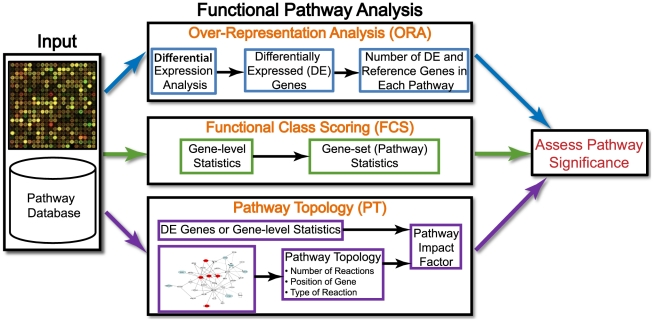
\includegraphics[width=1\linewidth]{images/fea_types} 

}

\caption{Types of  of functional enrichment analysis}\label{fig:unnamed-chunk-6}
\end{figure}

\emph{Source: Figure adapted from Khatri P, Sirota M, Butte AJ. Ten years of pathway analysis: current approaches and outstanding challenges. PLoS Comput Biol. 2012;8(2):e1002375.}

\hypertarget{over-representation-analysis-ora}{%
\subsection{Over Representation Analysis (ORA)}\label{over-representation-analysis-ora}}

Over Representation Analysis (ORA) is one of the simplest and most widely used methods for functional enrichment analysis. ORA aims to determine whether specific biological categories (e.g., pathways, Gene Ontology terms) are statistically overrepresented in a given list of features (like genes or proteins) compared to a background or reference set. This method focuses on counting the number of features from the list that are associated with a specific category and comparing this count to what would be expected by chance.

\hypertarget{input-data}{%
\subsubsection{Input Data}\label{input-data}}

\begin{itemize}
\item
  {List of Features:} This refers to the subset of biomolecules identified as significantly regulated or altered in the study. Features might include genes, proteins, lipids, or other biomolecules, depending on the type of -omics data.
\item
  {Background Set:} The background set, or universe, consists of all the features that were measured in the study or a defined subset of the total genome, proteome, or metabolome being studied. The background is critical for enrichment analysis because it provides the context against which the significance of feature enrichment is assessed.
\end{itemize}

\hypertarget{workflow}{%
\subsubsection{Workflow}\label{workflow}}

{How it works}: ORA uses a predefined feature list (e.g., from differentially expressed genes), calculates the number of features in the list that belong to a certain category (e.g., a pathway), and tests whether this number is significantly higher than expected using statistical tests like the hypergeometric test or Fisher's exact test.

{Strengths}: Simple and easy to implement. Works well with a predefined list of significant features.

{Limitations}: ORA does not take into account the full range of feature expression values and can miss subtle changes across a broader set of features. It relies heavily on selecting a predefined cut-off to create the feature list, which can be subjective.

\hypertarget{gene-set-enrichment-analysis-gsea}{%
\subsection{Gene Set Enrichment Analysis (GSEA)}\label{gene-set-enrichment-analysis-gsea}}

Gene Set Enrichment Analysis (GSEA) also known as Functional Class Scoring (FCS) is a more sophisticated method that avoids the need to define a strict cut-off for selecting a list of significant features. Instead of using a discrete list of differentially expressed features, GSEA analyses ranked feature expression data. It evaluates whether predefined gene sets (such as pathways or functional categories) are enriched at the top or bottom of the ranked list, capturing subtle but coordinated changes in gene expression.

\hypertarget{input-data-1}{%
\subsubsection{Input Data}\label{input-data-1}}

\begin{itemize}
\item
  {Ranked List:} In some enrichment methods, such as Gene Set Enrichment Analysis (GSEA), a ranked list is used instead of a simple feature list. The ranking is typically based on a continuous metric such as the magnitude of gene expression changes or some sort of statistical test output. This ranked list helps prioritise features that exhibit the strongest biological relevance and facilitates more nuanced enrichment analyses that consider the direction and strength of biomolecular changes.
\item
  {Gene Sets:} This refers to predefined groups of genes that share a common biological property, such as involvement in a specific biological pathway, functional category, or regulatory process. The most commonly used format for gene sets in MSigDB is the GMT format. This format is simple, human-readable, and widely supported by various GSEA tools.
\end{itemize}

\hypertarget{workflow-1}{%
\subsubsection{Workflow}\label{workflow-1}}

{How it works}: GSEA first ranks all genes in the dataset according to their differential expression levels (e.g., from a control to a condition). Then, for each predefined gene set, it calculates an enrichment score (ES) that reflects the concentration of the gene set members at the extremes of the ranked list. Statistical significance is assessed through permutation testing, and the False Discovery Rate (FDR) is used to correct for multiple comparisons.

{Strengths}: GSEA avoids arbitrary thresholds for feature selection and can detect coordinated changes across sets of genes, even if individual genes within the set do not show significant differential expression.

{Limitations}: GSEA may miss smaller pathways or functional categories if their features are not highly ranked or uniformly expressed. It is also more computationally intensive than ORA.

\hypertarget{pathway-topology-pt-based-enrichment}{%
\subsection{Pathway Topology (PT)-Based Enrichment}\label{pathway-topology-pt-based-enrichment}}

Pathway Topology (PT)-based enrichment analysis extends beyond merely counting features and instead incorporates the topological structure of biological pathways. This method evaluates not only which features are part of a pathway but also their position and interactions within the pathway. By considering the connectivity and interaction strength between features, PT-based approaches provide a more biologically meaningful interpretation of pathway activation or suppression.

\hypertarget{input-data-2}{%
\subsubsection{Input Data}\label{input-data-2}}

\begin{itemize}
\tightlist
\item
  {List of Features or Ranked List:} Already explained.
\item
  {Pathway Topology:} This refers to the structure of a biological pathway, which includes detailed information about the interactions and relationships between gene products (such as proteins or RNAs) within a pathway.
\end{itemize}

\hypertarget{workflow-2}{%
\subsubsection{Workflow}\label{workflow-2}}

{How it works}: PT-based methods take into account the direction and magnitude of feature expression changes, as well as the structure of pathways (e.g., signaling cascades, metabolic pathways). They consider how biomolecule products interact with one another and the specific roles of each gene within the pathway. Topological factors like the number of connections a gene has or its centrality in the pathway are considered when assessing the enrichment.

{Strengths}: Provides more biologically relevant insights by considering gene-gene interactions and the position of each gene within a pathway. It is particularly useful for complex pathways where the roles of genes differ based on their interactions with others.

{Limitations}: Requires more detailed pathway annotations and higher computational complexity. Pathway databases may not have complete or accurate topological information for all pathways, limiting the analysis for certain datasets.

PT-based enrichment will be covered in this workshop:
Given the focus of this workshop on more widely used and accessible enrichment methods, PT-based analysis will not be covered for its limited practical applications (primarily due to the insufficient availability of comprehensive and well-annotated pathway topology databases). Instead, we will focus on methods like ORA and GSEA, which are better supported by existing databases and easier to apply in typical omics studies. However, participants are encouraged to explore PT-based enrichment in the future as database resources improve.

\hypertarget{annotation-databses}{%
\section{Annotation Databses}\label{annotation-databses}}

Functional annotation databases are curated collections of biological data that systematically categorise and describe the functions, roles, interactions, and pathways of genes, proteins, or other biological molecules, enabling researchers to link experimental data to biological knowledge.

\hypertarget{go-gene-ontology}{%
\subsection{\texorpdfstring{\href{https://geneontology.org/}{GO: Gene Ontology}}{GO: Gene Ontology}}\label{go-gene-ontology}}

``The goal of the Gene Ontology Consortium is to produce a dynamic, controlled vocabulary that can be applied to all eukaryotes even as knowledge of gene and protein roles in cells is accumulating and changing.'' (Ashburner et al.~2000)

\begin{figure}

{\centering 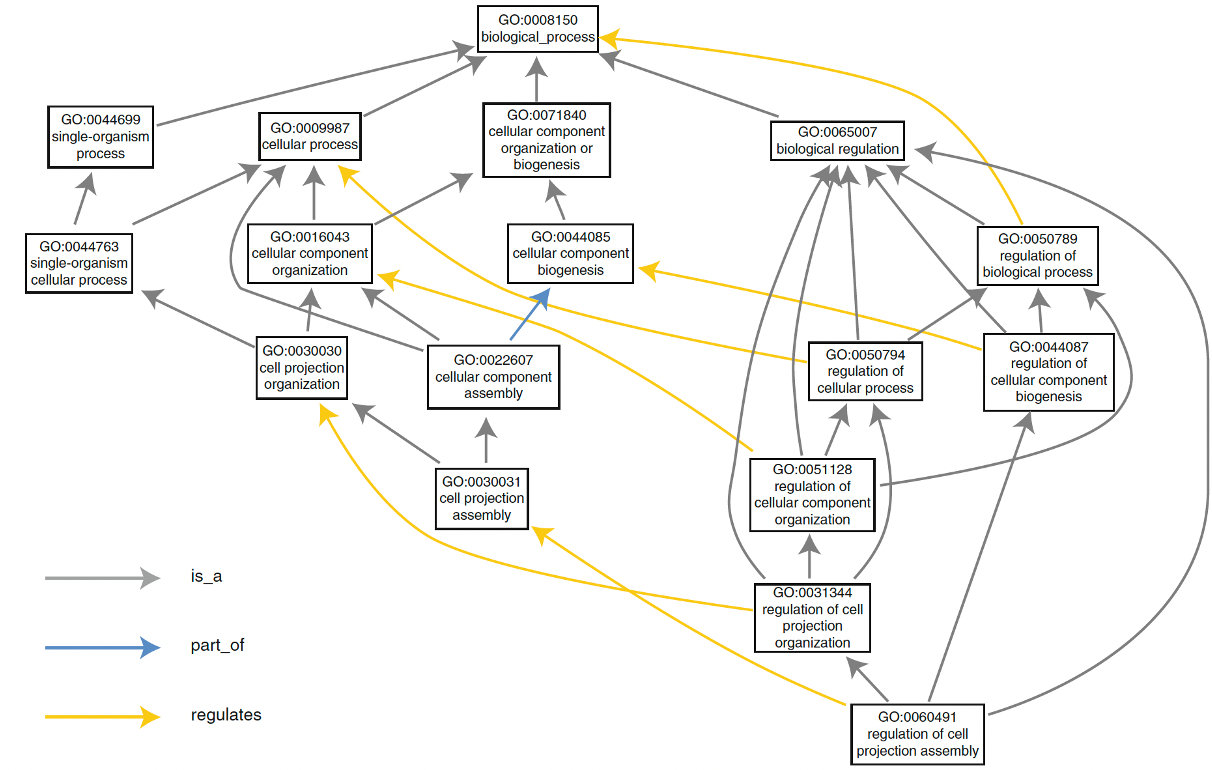
\includegraphics[width=1\linewidth]{images/go_structure} 

}

\caption{The structure of gene ontology.}\label{fig:unnamed-chunk-7}
\end{figure}

\emph{Imagen source \href{https://link.springer.com/book/10.1007/978-1-4939-3743-1}{The Gene Ontology Handbook}}

Gene Ontology (GO) is a structured framework used to describe the roles of genes and their products across all living organisms. It provides a controlled vocabulary that allows for consistent descriptions of gene functions, biological processes, and cellular locations, facilitating computational analysis and integration of biological data across different species. GO's structure comprises three main aspects:

{1. Molecular Function:}
In the Gene Ontology (GO), molecular function refers to the specific biochemical activity that a gene product (such as a protein or RNA) performs. This activity typically involves direct physical interactions with other molecular entities, such as catalysis or binding. These functions are described based on their biochemical roles (e.g., enzyme activity) and their contribution as components within larger biological systems. For instance, protein kinase activity involves the phosphorylation of proteins, which is a specific molecular function. In GO, molecular function is concerned with the direct action of gene products, whether in terms of biochemical interactions or roles in larger biological systems.

{2. Biological Process:}
Biological processes represent the larger objectives that gene products contribute to in an organism, often described by the outcome or result of a series of molecular events. These processes are broader, coordinated sequences of molecular activities that achieve a biological objective, such as cell division or DNA replication. A biological process in GO can encompass anything from simple enzymatic actions to complex, regulated systems like embryonic development or immune response. GO annotations aim to associate gene products not only with the processes they directly contribute to but also with processes they regulate or enable.

{3. Cellular Component:}
This aspect of GO refers to the specific location within a cell where a gene product operates. Cellular components are described relative to structures within the cell, such as the mitochondrion or plasma membrane, and reflect where molecular functions occur as part of broader biological processes. These locations are vital to understanding where molecular activities take place, as cellular compartmentalisation often influences the function and regulation of gene products. Unlike molecular function and biological process, cellular components refer more to cellular anatomy, specifying where gene products perform their roles during biological activities.

In practice, GO terms and annotations allow researchers to describe gene functions in a standardised way, helping in tasks such as gene function prediction, functional profiling, and comparing genes across species. GO's hierarchical organisation of terms provides a rich framework to model the complexity of biological systems and facilitates the computational study of gene functions.

\hypertarget{kegg-kyoto-encyclopedia-of-genes-and-genomes}{%
\subsection{\texorpdfstring{\href{https://www.genome.jp/kegg/}{KEGG: Kyoto Encyclopedia of Genes and Genomes}}{KEGG: Kyoto Encyclopedia of Genes and Genomes}}\label{kegg-kyoto-encyclopedia-of-genes-and-genomes}}

Kyoto Encyclopedia of Genes and Genomes (KEGG) is a curated database that integrates genomic, chemical, and systemic information to represent biological systems and their interactions. It allows users to map molecular data (such as genes, proteins, and small molecules) to biological pathways, enabling a better understanding of how different components interact within an organism.

\begin{figure}

{\centering 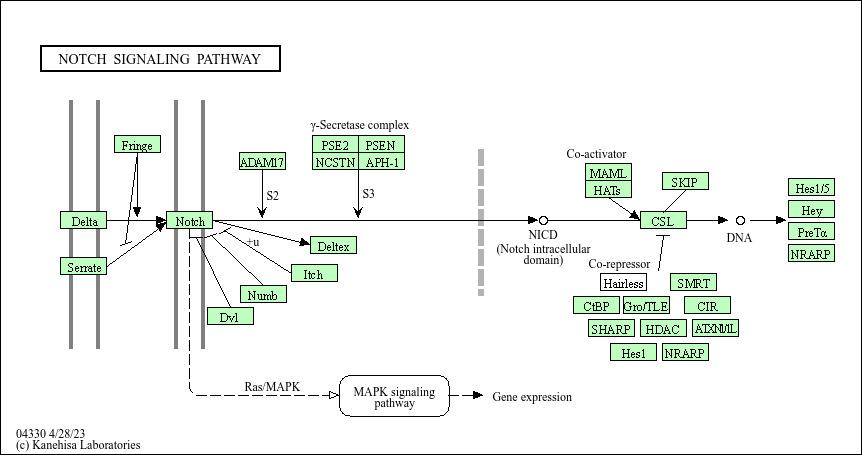
\includegraphics[width=1\linewidth]{images/NOTCH_signaling_pathway_kegg} 

}

\caption{NOTCH Signaling Pathway by KEGG}\label{fig:unnamed-chunk-8}
\end{figure}

\hypertarget{reactome}{%
\subsection{\texorpdfstring{\href{https://reactome.org/}{Reactome}}{Reactome}}\label{reactome}}

Reactome pathway knowledgebase is an open-access, manually curated database that captures molecular details of biological processes such as signal transduction, DNA replication, metabolism, and more, using a consistent data model across different domains of biology. This makes it particularly well-suited for functional enrichment analysis, where understanding the relationships between gene expression data and biological pathways is crucial.

\begin{figure}

{\centering 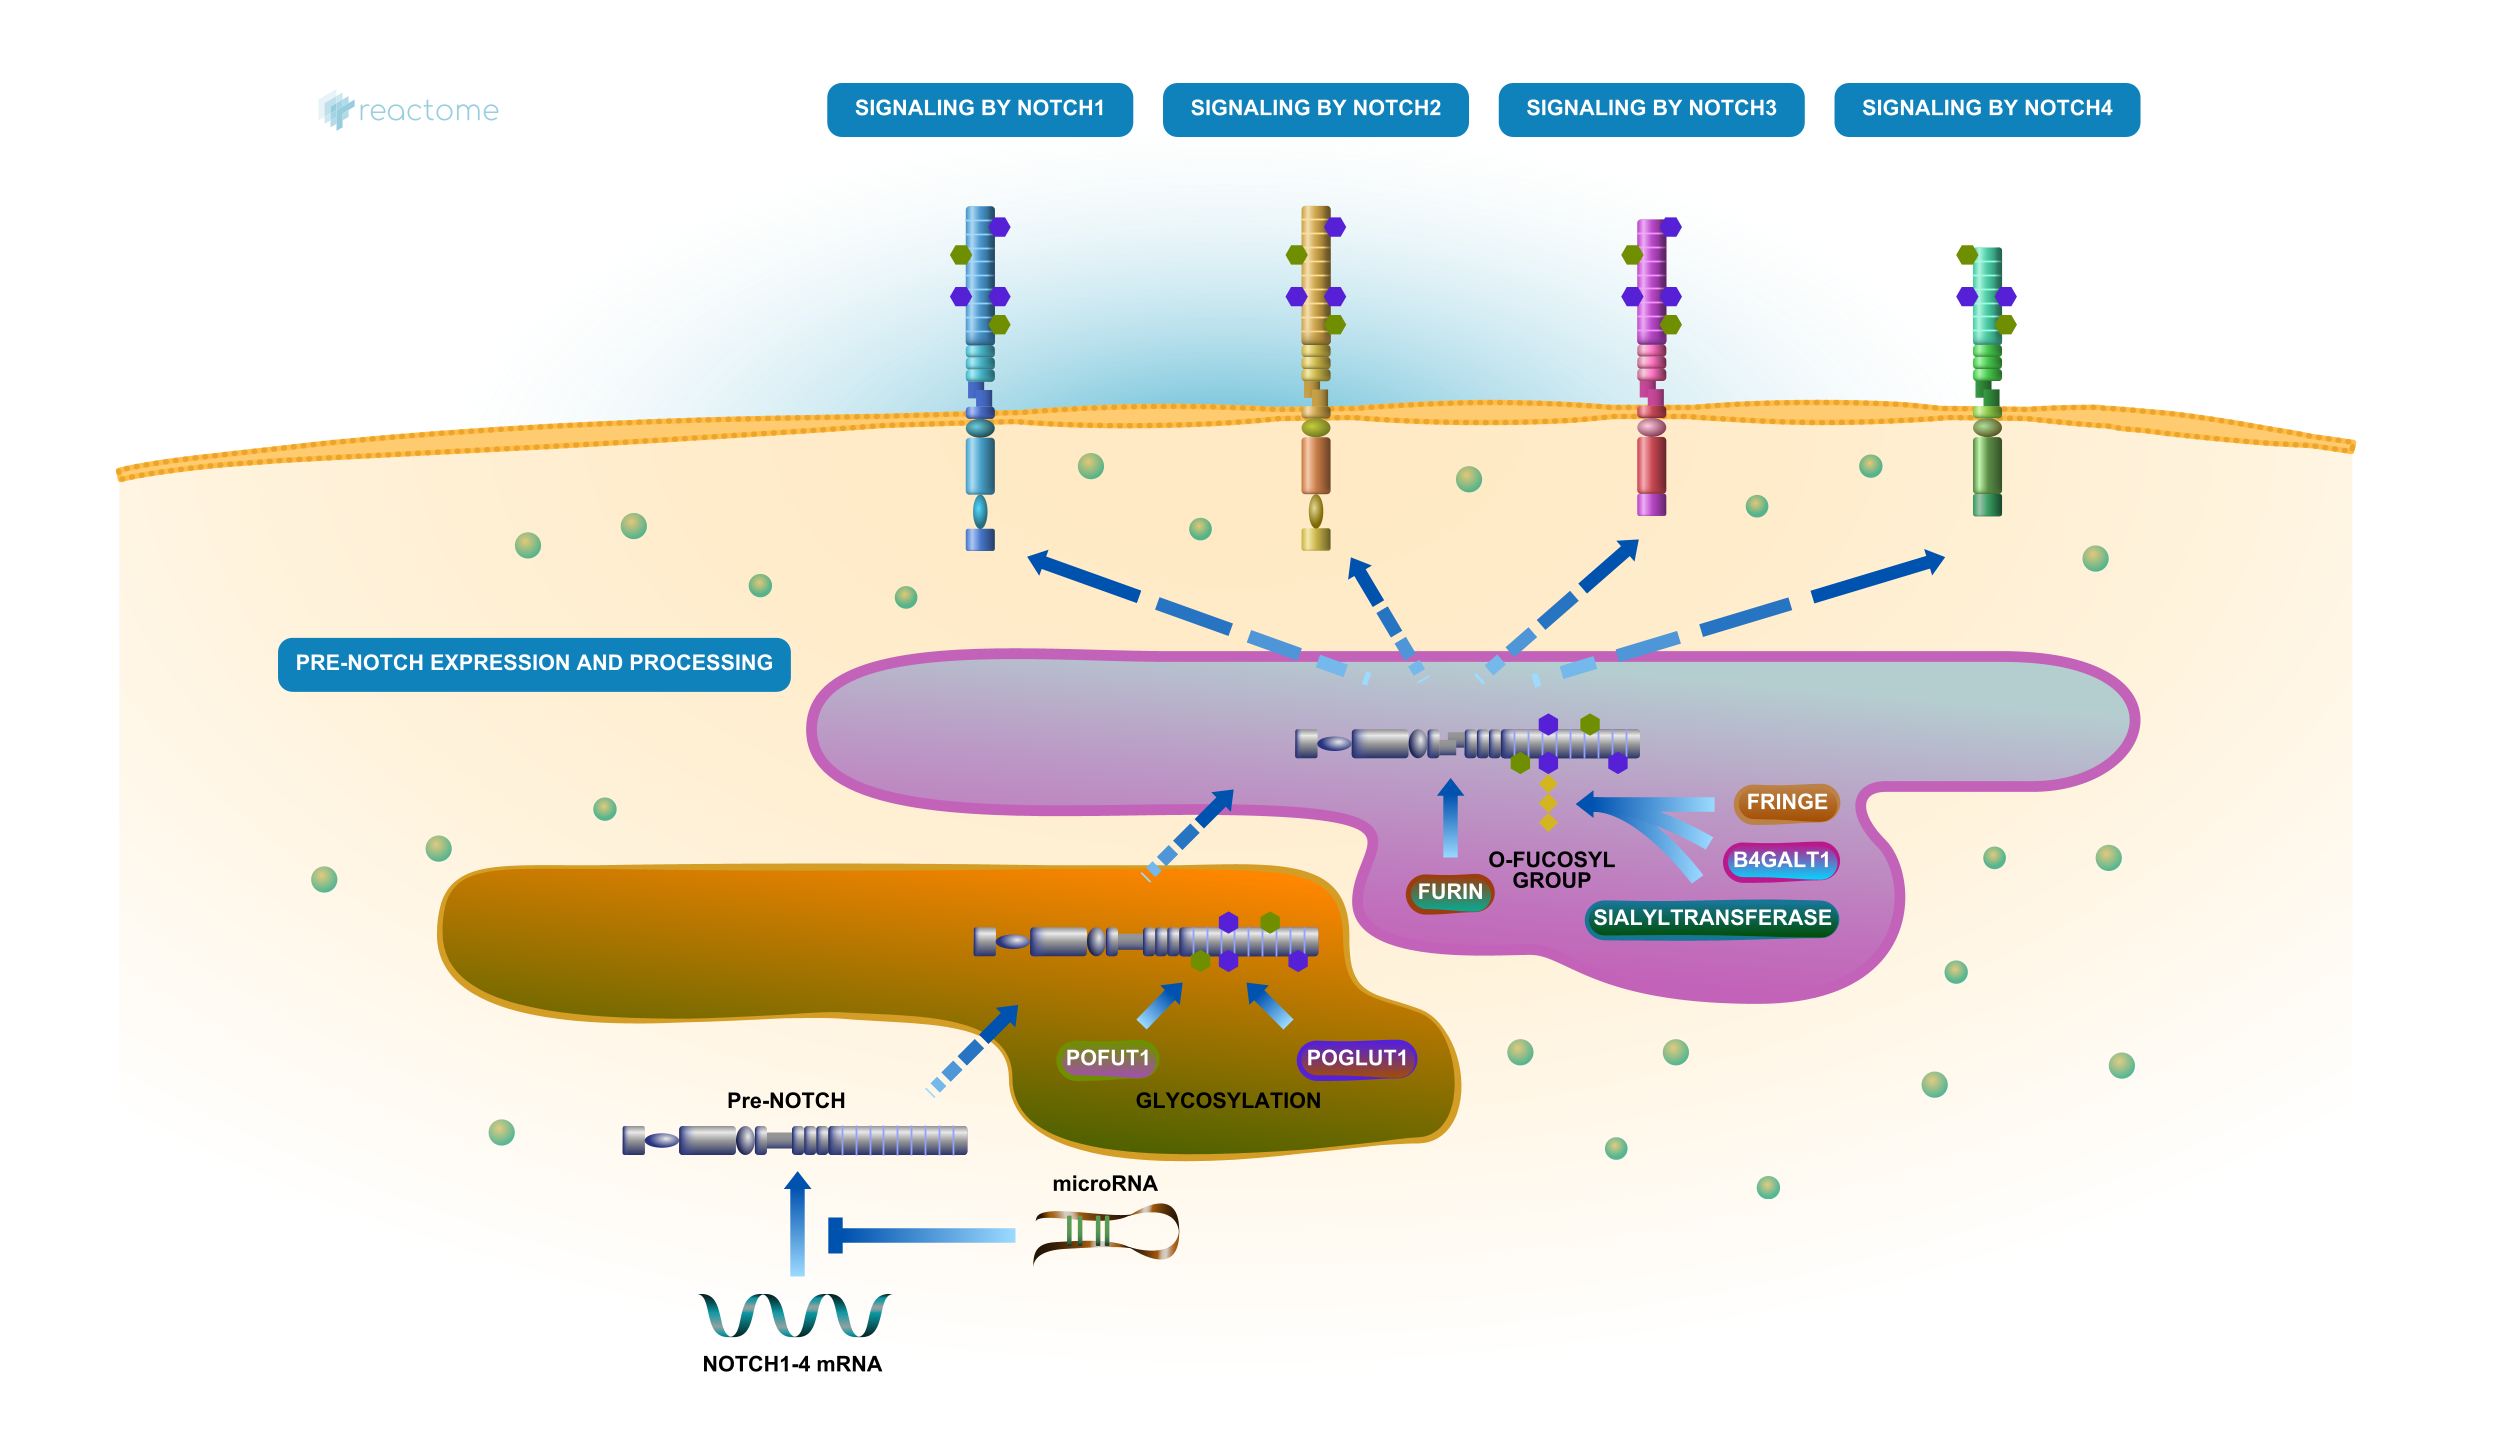
\includegraphics[width=1\linewidth]{images/NOTCH_signaling_pathway_reactome} 

}

\caption{NOTCH Signaling Pathway by Reactome}\label{fig:unnamed-chunk-9}
\end{figure}

\hypertarget{msigdb}{%
\subsection{\texorpdfstring{\href{https://www.gsea-msigdb.org/}{MSigDB}}{MSigDB}}\label{msigdb}}

Molecular Signatures Database (MSigDB) is a comprehensive resource for gene set enrichment analysis. It offers a comprehensive collection of gene sets that represent biological processes, molecular pathways, and other biologically relevant information. MSigDB is integrated with the Gene Set Enrichment Analysis (GSEA) tool, which is commonly used to determine if predefined sets of genes show statistically significant differences between two biological states (e.g., diseased vs.~healthy samples).

\begin{figure}

{\centering \includegraphics[width=1\linewidth]{images/GSEA-homegraphic} 

}

\caption{GSEA Workflow}\label{fig:unnamed-chunk-10}
\end{figure}

\hypertarget{common-tools-for-doing-fea}{%
\section{Common Tools for Doing FEA}\label{common-tools-for-doing-fea}}

\hypertarget{enrichment-statistics}{%
\chapter{Enrichment Statistics}\label{enrichment-statistics}}

Enrichment statistics are based on a contingency table like so:

..in term

..not in term

Total

..in gene list

50

100

150

..not in gene list (but in background)

200

15900

16100

Total

250

16000

16250

This is based on the 16250 genes that were measured in your experiment.

Note that there might be extra genes that weren't measured these are excluded from the calculations entirely. E.g. There might have been an extra 5000 terms (some of which might have been annotated with the term of interest), making for 21250 \emph{annotated} genes.

\begin{center}\rule{0.5\linewidth}{0.5pt}\end{center}

\hypertarget{fishers-exact-test}{%
\section{\texorpdfstring{{Fisher's Exact Test}}{Fisher's Exact Test}}\label{fishers-exact-test}}

Fisher's Exact Test is a statistical test used to determine if there are nonrandom associations between the proportions of two categorical variables. It calculates the exact probability of observing the given distribution of counts in a 2x2 contingency table, under the null hypothesis of no association between the variables.

\begin{quote}
\emph{Note:} This is just a toy calculator for this training, it is quite limited. You can also use some online tools like \href{https://www.socscistatistics.com/tests/fisher/default2.aspx}{Social Science Statistics} to play with.
\end{quote}

\emph{Formula}:
\[P = \frac{(a + b)!(c + d)!(a + c)!(b + d)!}{a!b!c!d!N!}\]

Where:

\begin{itemize}
\item
  \(a\), \(b\), \(c\), and \(d\) are the observed counts in the 2x2 contingency table.
\item
  \(N\) is the total number of observations, \(N = a + b + c + d\).
\end{itemize}

Given this contingency table:

\begin{longtable}[]{@{}llll@{}}
\toprule\noalign{}
& Category 1 & Category 2 & Total \\
\midrule\noalign{}
\endhead
\bottomrule\noalign{}
\endlastfoot
\textbf{Group 1} & \(a\) & \(b\) & \(a + b\) \\
\textbf{Group 2} & \(c\) & \(d\) & \(c + d\) \\
\textbf{Total} & \(a + c\) & \(b + d\) & \(a + b + c + d\) \\
\end{longtable}

\emph{R syntax}

\hypertarget{hypergeometric-test}{%
\section{\texorpdfstring{{Hypergeometric Test}}{Hypergeometric Test}}\label{hypergeometric-test}}

Hypergeometric test calculates the probability of observing the given number of genes from a specific category (e.g., a pathway) in the gene list (differentially expressed genes) by chance. It models the situation where you draw a sample (the gene list) from a finite population (the background of all genes), and success is defined as a gene being in the category (e.g., belonging to the pathway).

\begin{quote}
\emph{Note:} Here is a tool by \href{https://stattrek.com/online-calculator/hypergeometric}{Stat Trek} to play around with the hypergeometric test.
\end{quote}

\emph{Formula:}
\[P(X = k) = \frac{\binom{K}{k} \binom{N - K}{n - k}}{\binom{N}{n}}\]
Where:

\begin{itemize}
\item
  \(N\) = Total number of items in the population.
\item
  \(K\) = Number of success items in the population.
\item
  \(n\) = Number of items in the sample.
\item
  \(k\) = Number of success items in the sample.
\end{itemize}

The parameters in our example:
N=16250; K=250; n=150; k=50

\emph{R syntax}

Where:

k−1 is the number of observed successes minus 1 (for the ``at least'' scenario).
lower.tail = FALSE gives the probability of getting at least k successes (right-tail).

\begin{center}\rule{0.5\linewidth}{0.5pt}\end{center}

\hypertarget{section}{%
\subsubsection*{}\label{section}}
\addcontentsline{toc}{subsubsection}{}

\hypertarget{activity}{%
\section{Activity}\label{activity}}

\hypertarget{challenge-interactive-calculator}{%
\subsection*{\texorpdfstring{\textbf{Challenge:} Interactive Calculator}{Challenge: Interactive Calculator}}\label{challenge-interactive-calculator}}
\addcontentsline{toc}{subsection}{\textbf{Challenge:} Interactive Calculator}

\href{https://bioinformatics3.erc.monash.edu/rsconnect/content/241/}{\emph{Link to open toy enrichment calculator}}.

This calculates enrichment for a single hypothetical genelist (e.g.~your RNAseq differentially expressed genelist) against a single hypothetical `term' (some set of interesting genes, e.g.~synaptic signaling genes). It makes a Venn diagram and a wordy description of what is being tested.

You can adjust various factors and see their effect on the enrichment p-values.

\hypertarget{section-1}{%
\subsubsection*{}\label{section-1}}
\addcontentsline{toc}{subsubsection}{}

\hypertarget{questions}{%
\subsection*{\texorpdfstring{\textbf{Questions}}{Questions}}\label{questions}}
\addcontentsline{toc}{subsection}{\textbf{Questions}}

\begin{enumerate}
\def\labelenumi{\arabic{enumi}.}
\tightlist
\item
  Is it significant at p=0.05?

  Show

  No, corrected pval=0.087
\item
  What about with a smaller background of 5000 genes (e.g.~proteomic datasets)?

  Show

  Even less so - corrected pval=1
\item
  Or, testing against a smaller database of terms; 2000 terms instead of 10000? With the original 16000 gene background.

  Show

  Yes, now corrected pval=0.017
\item
  19 out of 200 differentially expressed genes (9.5\%), need to hit for a 500-gene term (3.1\% of all genes) to be significant at (p=0.048). How many hits would be needed for a more specific 30-gene term?

  Show

  5 hits - 2.5\% of the differentially expressed genes vs 0.19\% of all genes
\end{enumerate}

\hypertarget{section-2}{%
\subsubsection*{}\label{section-2}}
\addcontentsline{toc}{subsubsection}{}

\hypertarget{example-analysis}{%
\chapter{Example Analysis}\label{example-analysis}}

\hypertarget{sh-sy5y-differentiation}{%
\section{SH-SY5Y Differentiation}\label{sh-sy5y-differentiation}}

SH-SY5Y is a commonly used neuroblastoma cell line.
With appropriate treatment, it can be induced to differentiate into a `more neuronal' form.
Differentiated cells look quite different, growing thin neurites out from the body of the cell.

\begin{figure}

{\centering 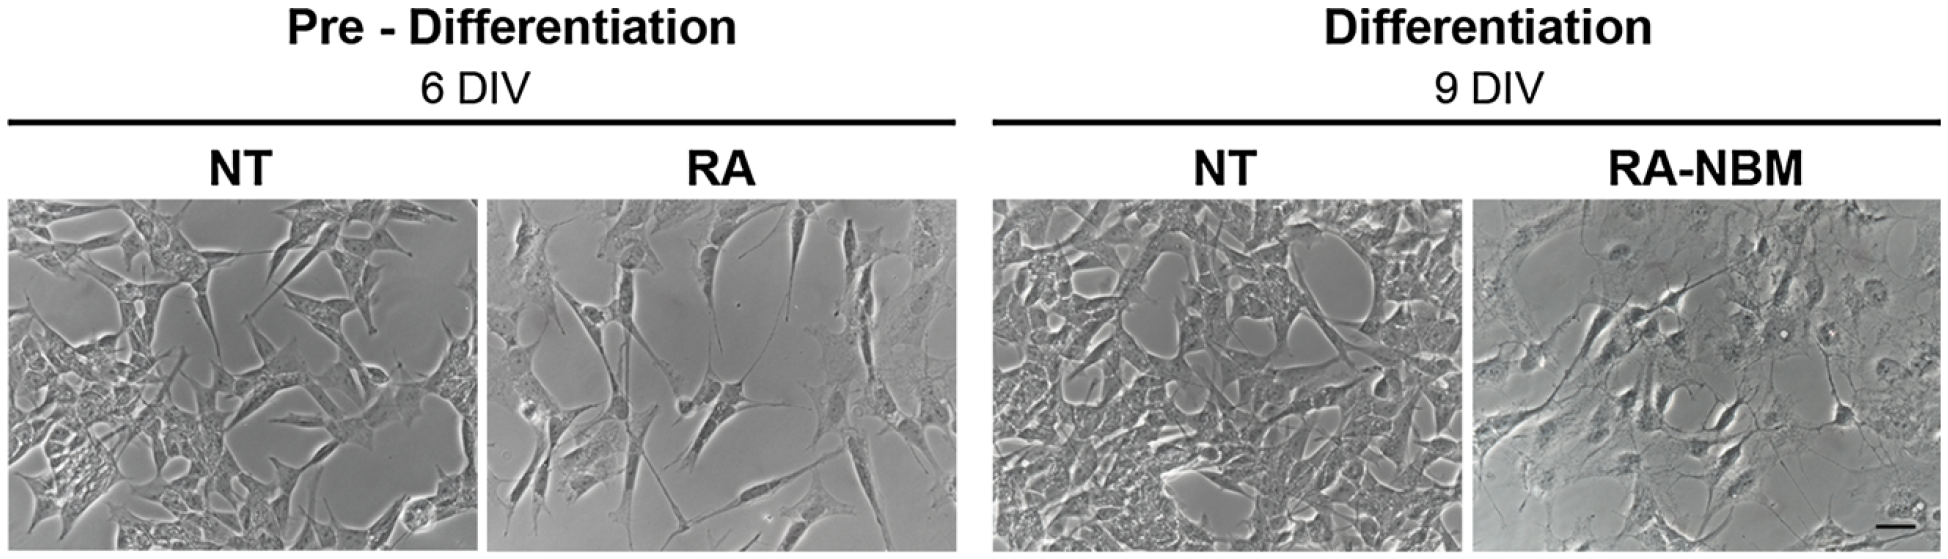
\includegraphics[width=1\linewidth]{images/shsy5ydiff} 

}

\caption{Morphological analysis of differentiated SH-SY5Y cells.<br>At 6-DIV stage, the cells exposed to RA showed an elongated morphology as compared to basal medium (NT). Cells subsequently treated in NBM for 3 days became more polarised, exhibited several neurites and branches and acquired a neuronal-like shape<br><br>Image is derived from Figure 4 (Pezzini et al. 2017).}\label{fig:unnamed-chunk-15}
\end{figure}

\hypertarget{the-question-what-pathways-are-involved-in-sh-sy5y-differentiation}{%
\section{The question: What pathways are involved in SH-SY5Y Differentiation?}\label{the-question-what-pathways-are-involved-in-sh-sy5y-differentiation}}

In their paper \href{https://link.springer.com/article/10.1007\%2Fs10571-016-0403-y}{\emph{Transcriptomic Profiling Discloses Molecular and Cellular Events Related to Neuronal Differentiation in SH-SY5Y Neuroblastoma Cells}}, Pezzini et al.~induced neuronal differentiation of the SH-SY5Y neuroblastoma cell line and measured transcriptomic changes using RNA sequencing (Pezzini et al.~2017). During the 9-day differentiation protocol, SH-SY5Y cells were initially pre-differentiated in a retinoic acid (RA) medium for 6 days, followed by a 3-day treatment with a neurobasal medium (NBM) enriched with neurotrophic factors. Control cells, which were not treated (NT), were maintained under basal conditions and served as a comparison group. The authors then performed functional enrichment analysis on the differentially expressed genes.

\hypertarget{the-data-differentially-expressed-genes}{%
\section{The data : Differentially expressed genes}\label{the-data-differentially-expressed-genes}}

The example dataset for today is the RNAseq differential expression results.

They can be accessed via this \href{http://degust.erc.monash.edu/degust/compare.html?code=5b2c7805ab8f8c5f2dc8c72e61b049b0\#?plot=mds}{Degust} link:

This has been reanalysed from the published raw data, via the degust tool.

\begin{quote}
\textbf{Note:} Other tools and approaches may produce different-looking results, but generally, you will end up with a table of genes containing some measure of statistical confidence. The methods for functional enrichment analysis should remain similar.
\end{quote}

\hypertarget{defining-the-genelist}{%
\chapter{Defining the genelist}\label{defining-the-genelist}}

Starting from those differential expression results \href{http://degust.erc.monash.edu/degust/compare.html?code=5b2c7805ab8f8c5f2dc8c72e61b049b0\#?plot=mds}{here}, how do we go about getting a genelist to calculate enrichment on?

\hypertarget{activities}{%
\section{Activities}\label{activities}}

Todays exercise follows the process of getting the differentially expressed gene list using excel. You could use another spreadsheet program, or some may prefer a programming language like R .

\begin{enumerate}
\def\labelenumi{\arabic{enumi}.}
\item
  Download the full table of data from either degust, or the csv file here:
  \href{https://monashbioinformaticsplatform.github.io/enrichment_analysis_workshop/data/Pezzini2016_SHSY5Ycelldiff_DE_table.csv}{Pezzini2016\_SHSY5Ycelldiff\_DE\_table.csv}. Import into excel.
\item
  How many genes are differentially expressed? In these results the FDR Column contains the corrected p-value, and the `differentiated' column shows the log2 fold-change of differentiated cells vs untreated cells (log2(diff)-log2(undiff)); 0 is unchanged, 1 is doubled, -1 is halved.

  \begin{itemize}
  \item
    Significant at 0.01?
  \item
    That's a particularly large number of genes - perhaps not unexpected given how much the cells are changed this experiment. How many significant genes also have 2-fold change in expression?
  \item
    For this workshop, get the genes with a FDR \textless1x10\^{}-4 and 2x fold change. Note that this is a ridiculous threshold - most experiments yeild far less differential expression, but the difference between these two cell conditions is pretty extreme! Typically you would only filter at p\textless0.01 (and occasionally 2-fold change) - you might see 10s to 100s of results. However, this arbitrary threshold gives a more typical number of differentially expressed genes for downstream analysis. An alternative approach could be to take the top 500 genes.
  \end{itemize}
\end{enumerate}

Show

There are 4923 differentially expressed genes, 2149 of which have a 2-fold change in expression. With the aggressive filtering, there are 198 genes left.

\begin{enumerate}
\def\labelenumi{\arabic{enumi}.}
\setcounter{enumi}{2}
\tightlist
\item
  How many genes are \emph{tested}? This is your background.
\end{enumerate}

Show

14420 genes tested.

\begin{center}\rule{0.5\linewidth}{0.5pt}\end{center}

\hypertarget{common-gotcha}{%
\section{Common gotcha}\label{common-gotcha}}

Can you find SEPT4? Because \href{https://genomebiology.biomedcentral.com/articles/10.1186/s13059-016-1044-7}{\emph{Gene name errors are widespread in the scientific literature}}

You can't revert the gene names automatically (try converting it to text!). You have to avoid it in the first place by importing gene columns as `text' columns in excel. See video from HUGO : \url{https://www.genenames.org/help/faq/\#!/\#tocAnchor-1-25-1}

\begin{center}\rule{0.5\linewidth}{0.5pt}\end{center}

\hypertarget{example}{%
\section{Example}\label{example}}

An example excel document showing this filtering process is here: \href{https://monashbioinformaticsplatform.github.io/enrichment_analysis_workshop/data/Pezzini2016_SHSY5Ycelldiff_DE_table_filtering.xlsx}{Pezzini2016\_SHSY5Ycelldiff\_DE\_table\_filtering.xlsx}.

\hypertarget{online-tools}{%
\chapter{Online Tools}\label{online-tools}}

Functional enrichment analysis can be performed using various web-based tools, each of which is designed to meet specific analytical needs. These tools often vary in the databases they use, their statistical approaches, and their capabilities to perform different types of analysis, such as Over-Representation Analysis (ORA) or Gene Set Enrichment Analysis (GSEA).

In this workshop, we will explore several popular tools for functional enrichment analysis, including gProfiler, STRING, Reactome, and MSigDB GSEA. Each tool offers unique features and insights, providing flexibility in selecting the right method for diverse datasets and research questions.

\hypertarget{fea-in-gprofiler}{%
\section{\texorpdfstring{FEA in gProfiler }{FEA in gProfiler }}\label{fea-in-gprofiler}}

gProfiler is known for its integration of numerous species and databases. It supports both ORA and GSEA, enabling users to assess Gene Ontology (GO), biological pathways, regulatory motifs and protein databases. With gProfile one can

\hypertarget{steps-to-perform-ora-in-gprofiler}{%
\subsection{Steps to perform ORA in g:Profiler:}\label{steps-to-perform-ora-in-gprofiler}}

{- Prepare Input List:} Ensure your input is formatted as one gene per line or in a suitable format for g:Profiler.

{- Input Gene List:} Paste your prepared gene list directly into the input box on the g:Profiler web page or upload a file containing your list.

{- Select Organism:} Choose the appropriate organism from the \texttt{Organism} dropdown menu (e.g., \emph{Homo sapiens} for human data).

{- Choose Statistical Domain Scope:} Under \texttt{Advanced\ options}, select your preferred statistical background from the \texttt{Statistical\ domain\ scope} menu.If you choose ``Custom'' background, provide your custom background list by pasting or uploading the relevant file.

{- Set Significance Threshold:} Select the desired significance threshold method, such as \emph{g:SCS}, \emph{Bonferroni}, or \emph{Benjamini-Hochberg}.
- Specify the threshold value (e.g., 0.05, 0.1, etc.).

{- Select Functional Annotation Databases: } Navigate to the \texttt{Data\ sources} tab and choose one or more databases for analysis. Available options include:

\begin{itemize}
\tightlist
\item
  \emph{Gene Ontology (GO)}: Biological Process, Molecular Function, and Cellular Component.
\item
  \emph{KEGG Pathways}
\item
  \emph{Reactome Pathways}
\item
  \emph{WikiPathways}
\item
  \emph{TRANSFAC}
\item
  \emph{mirTarBase}
\item
  \emph{Human Protein Atlas}
\item
  \emph{CORUM}
\item
  \emph{Human Phenotype Ontology (HP)}
\end{itemize}

{- Run Query:} Run the analysis and review the enriched terms, pathways, and visual outputs. Download the results as needed for further exploration.

\hypertarget{browse-the-gprofiler-results}{%
\subsubsection{Browse the gProfiler Results}\label{browse-the-gprofiler-results}}

\begin{itemize}
\item
  \textbf{Overview}:
  The analysis provided a comprehensive list of enriched terms across selected databases, highlighting significant GO. The results give a high-level summary of pathways or terms most relevant to the input data.
\item
  \textbf{Detailed Results}:
  The detailed results section includes a tabulated format with enriched terms, adjusted p-values, and relevant statistics. Each entry provides information such as the enrichment score, associated genes, and functional annotations, allowing for an in-depth understanding of biological significance.
\item
  \textbf{GO Context}:
  The Gene Ontology (GO) context is divided into three main categories: Biological Process (BP), Molecular Function (MF), and Cellular Component (CC). The analysis identifies which GO terms are significantly enriched, offering insights into the broader biological implications of the gene set. This helps in pinpointing processes such as cellular responses, metabolic pathways, and molecular interactions.
\item
  \textbf{Query Info}:
  This section includes specifics about the input data, including the total number of queried genes and any identifiers not recognized or mapped. It also details the statistical background used, the chosen organism, and other analysis settings, ensuring transparency and reproducibility of the results.
\end{itemize}

\hypertarget{section-3}{%
\subsubsection*{}\label{section-3}}
\addcontentsline{toc}{subsubsection}{}

\hypertarget{different-backgrounds}{%
\subsubsection{Different Backgrounds}\label{different-backgrounds}}

\hypertarget{challenge-how-different-backgrounds-impact-the-output}{%
\subsubsection*{\texorpdfstring{\textbf{Challenge:} How different backgrounds impact the output?}{Challenge: How different backgrounds impact the output?}}\label{challenge-how-different-backgrounds-impact-the-output}}
\addcontentsline{toc}{subsubsection}{\textbf{Challenge:} How different backgrounds impact the output?}

Use `All known genes' in one analysis and `Custom' background in another. Download the results by clicking on CSV button. Browse the results in the spreadsheets and find out the difference between two.

\hypertarget{questions-1}{%
\subsubsection*{\texorpdfstring{\textbf{Questions }}{Questions }}\label{questions-1}}
\addcontentsline{toc}{subsubsection}{\textbf{Questions }}

Which background would you use in your analysis?

How is multi-query support implemented in gProfiler?

How can one perform Under Representation Analysis in gProfiler?

\hypertarget{steps-to-perform-gsea-in-gprofiler}{%
\subsection{Steps to perform GSEA in g:Profiler:}\label{steps-to-perform-gsea-in-gprofiler}}

{- Prepare Your Pre-ranked List:} Steps to provide a ranked gene list are given \href{degust.html}{here}.

{- Input Gene List:} Paste your prepared gene list directly into the input box on the g:Profiler web page or upload a file containing your list.

{- Select Organism:} Same as above.

{- Select Ordered query:} The ``Ordered query'' option in g:Profiler is designed to work with pre-ranked gene lists.

{- Set Significance Threshold:} Same as above.

{- Provide a Custom GMT:} This GMT file can be downloaded from \href{https://www.gsea-msigdb.org/gsea/msigdb/index.jsp}{MSigDB}.

{- Run Query:} Same as above.

\hypertarget{challenge-gsea-with-gprofiler}{%
\subsubsection*{\texorpdfstring{\textbf{Challenge:} GSEA with gProfiler}{Challenge: GSEA with gProfiler}}\label{challenge-gsea-with-gprofiler}}
\addcontentsline{toc}{subsubsection}{\textbf{Challenge:} GSEA with gProfiler}

Download the Hallmark gene sets (\href{https://www.gsea-msigdb.org/}{h.all.v2024.1.Hs.symbols.gmt}) from MSigDB and use it as Custom GMT.

\hypertarget{question}{%
\subsubsection*{\texorpdfstring{\textbf{Question }}{Question }}\label{question}}
\addcontentsline{toc}{subsubsection}{\textbf{Question }}

How can one use multi-GMT as custom background?

\hypertarget{fea-in-string}{%
\section{\texorpdfstring{FEA in STRING }{FEA in STRING }}\label{fea-in-string}}

STRING (Search Tool for the Retrieval of Interacting Genes/Proteins) is a resource for exploring protein-protein interaction (PPI) networks. It combines experimental data, predictions, and curated information to build networks that highlight functional relationships, helping to reveal shared pathways or biological processes within gene or protein lists.

\hypertarget{steps-to-perform-ora-in-string}{%
\subsection{Steps to Perform ORA in STRING:}\label{steps-to-perform-ora-in-string}}

{- Select Multiple proteins tab.}

{- Input Gene List:} Paste your prepared gene list directly into the input box on the STRING web page or upload a file containing your list.

{- Select Organism:} Choose the appropriate organism from the \texttt{Organisms} dropdown menu (e.g., \emph{Homo sapiens} for human data). STRING would auto-detect the organism if ENSEMBL IDs provided.

{- Modify Settings:} Under \texttt{Advanced\ Settings}, you can modify \texttt{Required\ score} from low (0.15) to highest (0.9) confidence. Similarly \texttt{FDR\ stringency} and \texttt{Network\ type} can be selected.

NOTE: In cases where long list of features is provided, STRING may chnage some of its settings so that:

\begin{itemize}
\tightlist
\item
  the nodes will have a simplified (not 3D) design
\item
  previews of protein structures are not shown
\item
  the network edges show interaction confidence only
\end{itemize}

\hypertarget{browse-the-string-results}{%
\subsection{Browse the STRING Results}\label{browse-the-string-results}}

STRING generates multiple tabs as output, shown here:

\begin{figure}

{\centering 
\includegraphics[width=1\linewidth]{images/string-results-tabs} 

}

\caption{Results tabs in STRING}\label{fig:unnamed-chunk-18}
\end{figure}

\hypertarget{viewers}{%
\subsubsection{Viewers}\label{viewers}}

Under the \texttt{Viewers} tab, various visualisation layouts are available, with the Network option being the most notable and widely used.

\hypertarget{legend}{%
\subsubsection{Legend}\label{legend}}

The \texttt{Legend} tab offers a guide to the colors of nodes and edges, along with annotations for each individual query in the input list.

\begin{figure}

{\centering 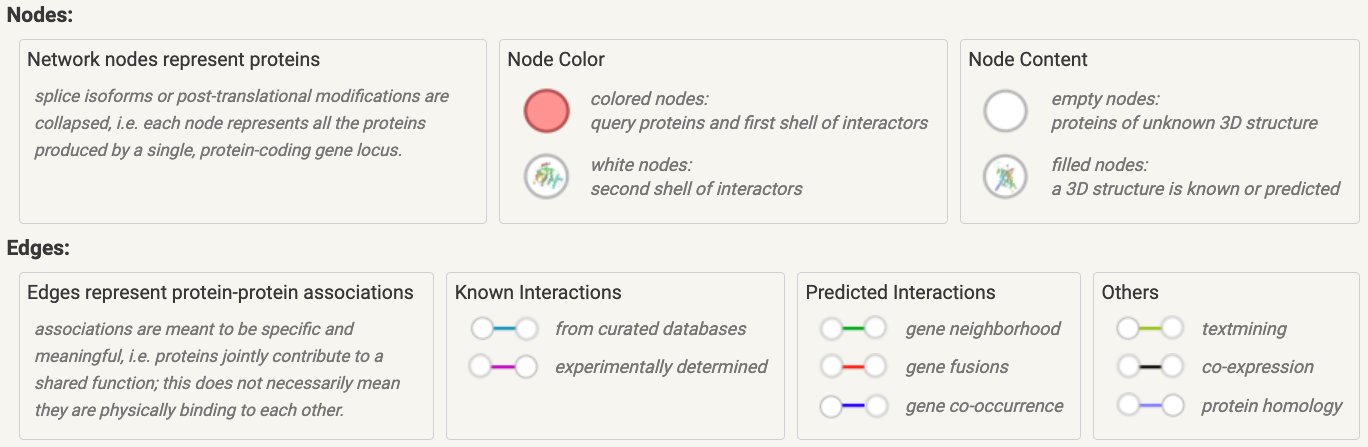
\includegraphics[width=1\linewidth]{images/string-legend} 

}

\caption{Nodes and edges colour-coded}\label{fig:unnamed-chunk-19}
\end{figure}

\hypertarget{settings}{%
\subsubsection{Settings}\label{settings}}

In the \texttt{Settings} tab of the STRING results, users have the flexibility to adjust existing settings and apply new filters to customise their data view and analysis. This tab you to switch between network types, strengths, data sources, intertaction scores and more.

\hypertarget{analysis}{%
\subsubsection{Analysis}\label{analysis}}

One of the most essential tabs is the \texttt{Analysis} tab, which offers comprehensive functional enrichment analysis from a range of databases. These include Gene Ontology (GO) for biological processes, molecular functions, and cellular components; Pathway enrichment from sources such as KEGG, Reactome, and WikiPathways; and other significant data sources such as Human Phenotype annotations and UniProt for protein function and structure.

Columns of the STRING enrichment table are explained as following:

{- Count In Network:}
The first number indicates how many proteins in your network are annotated with a particular term. The second number indicates how many proteins in total (in your network and in the background) have this term assigned. You can click on the numbers to see the network view of the gene sets behind them.

{- Strength:}
Log10(observed / expected). This measure describes how large the enrichment effect is. It's the ratio between i) the number of proteins in your network that are annotated with a term and ii) the number of proteins that we expect to be annotated with this term in a random network of the same size.

{- Signal:}
The signal is defined as a weighted harmonic mean between the observed/expected ratio and -log(FDR). FDR tends to emphasize larger terms due to their potential for achieving lower p-values, while the observed/expected ratio highlights smaller terms, which have a high foreground to background ratio but cannot achieve low FDR values due to their size. The signal measure seeks to balance both metrics for a more intuittive ordering of enriched terms.

{- False Discovery Rate:}
This measure describes how significant the enrichment is. Shown are p-values corrected for multiple testing within each category using the Benjamini--Hochberg procedure.

STRING visualises terms within each category using a bubble plot, effectively showcasing the significance and size of enriched terms. Additionally, it renders groups of related terms based on a user-defined similarity level, allowing users to identify clusters of functionally related terms within the data. This helps in interpreting complex enrichment results and highlighting key biological processes or pathways that are closely associated.

\begin{figure}

{\centering 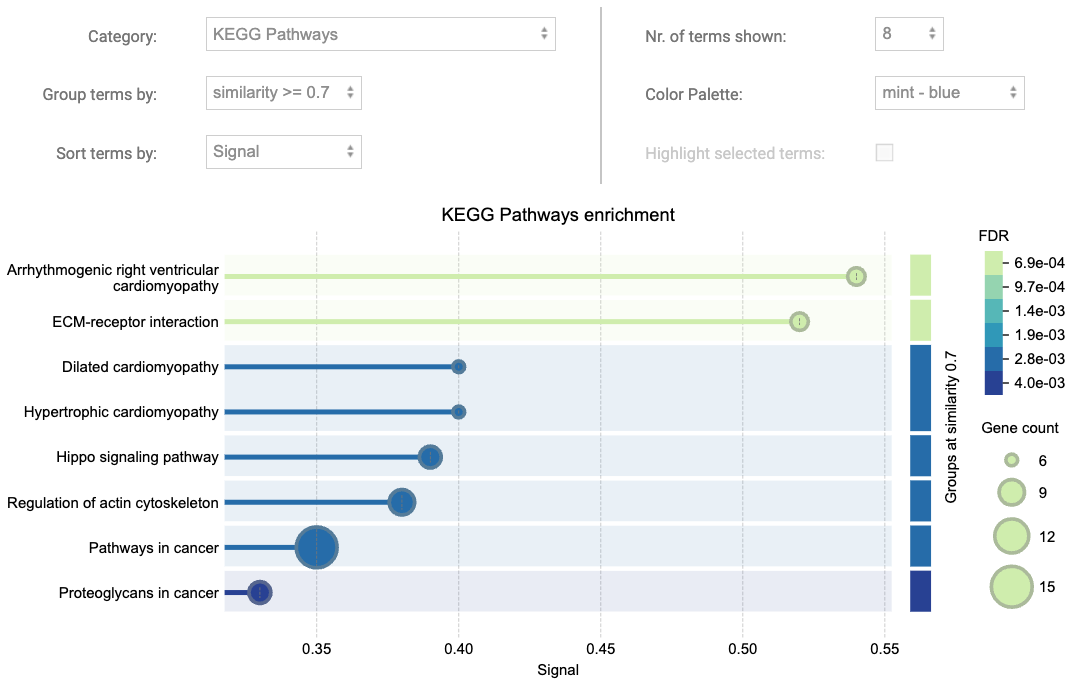
\includegraphics[width=1\linewidth]{images/string-enrichment_KEGG_sim0.7_graph_plus} 

}

\caption{Functional enrichment visualisation with STRING}\label{fig:unnamed-chunk-20}
\end{figure}

Towards the the bottom of the \texttt{Analysis} page, one can change the background including adding one of their own.

\begin{figure}

{\centering 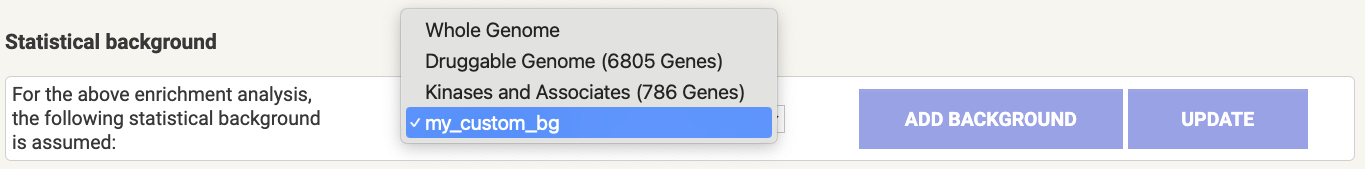
\includegraphics[width=1\linewidth]{images/string-statistical-background} 

}

\caption{Statistical background}\label{fig:unnamed-chunk-21}
\end{figure}

Finally the enriched terms can be downloaded at the end of the \texttt{Analysis} page, either individually per category or all enriched terms together.

\hypertarget{exports}{%
\subsubsection{Exports}\label{exports}}

The network data can be exported with the \texttt{Exports} tab. Also Network data can be directly sent to \href{https://cytoscape.org/}{Cytoscape} 
\includegraphics{images/network-to-Cytoscape.png} for further networking. It is expected to have Cytoscape installed before exporting to it.

\hypertarget{clusters}{%
\subsubsection{Clusters}\label{clusters}}

The \texttt{Clusters} tab essentially provides three different types of clustering algorithms:

\begin{itemize}
\item
  k-means clustering: Initialise \emph{k} centroids randomly, assigns each data point to the nearest centroid, recompute the centroids as the mean of all points in a cluster until until centroids do not change significantly.
\item
  MCL clustering (Markov clustering): is a graph-based algorithm that uses flow simulation to detect clusters in a network by modeling random walks.
\item
  DBSCAN clustering: is a density-based algorithm that groups points closely packed together while marking points in low-density regions as outliers or noise
\end{itemize}

\begin{figure}

{\centering 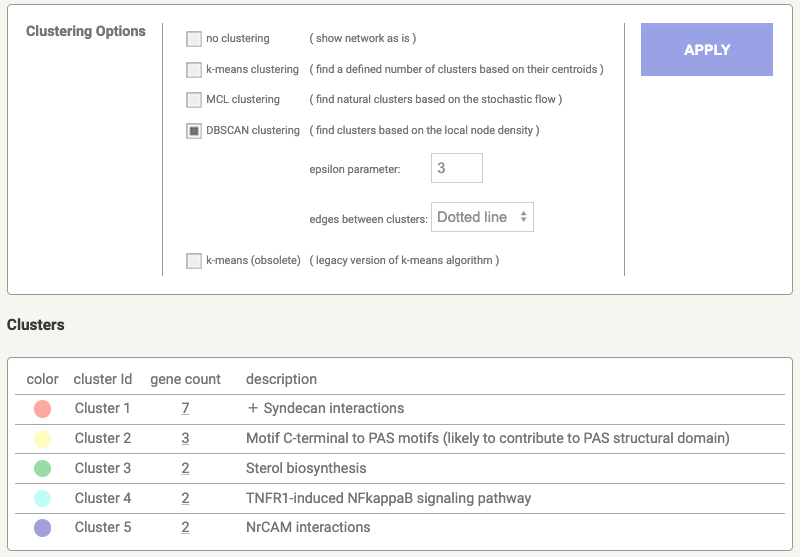
\includegraphics[width=1\linewidth]{images/string-clusters} 

}

\caption{Network clustering in STRING}\label{fig:unnamed-chunk-22}
\end{figure}

Clusters can be downloaded in \texttt{.tsv} format.

\hypertarget{question-1}{%
\subsubsection*{\texorpdfstring{\textbf{Question}}{Question}}\label{question-1}}
\addcontentsline{toc}{subsubsection}{\textbf{Question}}

What was the overlap in enrichment terms between gProfiler and STRING at FDR ≤ 0.05?

\hypertarget{fea-in-genepattern}{%
\section{\texorpdfstring{FEA in GenePattern }{FEA in GenePattern }}\label{fea-in-genepattern}}

GenePattern, an online platform developed by the Broad Institute, offers a suite of tools for analyzing and visualizing genomic data, making bioinformatics accessible to researchers through a user-friendly, no-programming interface. Among its supported tools is Gene Set Enrichment Analysis (GSEA), which implements \href{https://www.gsea-msigdb.org/gsea/index.jsp}{MSigDB GSEA} analysis for identifying enriched gene sets in genomic data.

MSigDB (Molecular Signatures Database) is a collection of gene sets for Gene Set Enrichment Analysis, representing pathways and gene signatures linked to biological states or diseases. It helps identify enriched gene sets, aiding the analysis of gene expression changes and key pathways in experimental data.

\hypertarget{steps-to-locate-gsea-module-in-genepattern}{%
\subsection{Steps to Locate GSEA Module in GenePattern:}\label{steps-to-locate-gsea-module-in-genepattern}}

\begin{itemize}
\tightlist
\item
  Click on the Run button and then the Public Server
\end{itemize}

\begin{figure}

{\centering 
\includegraphics{images/GenePattern-Run} 

}

\caption{Navigate to Public Server}\label{fig:unnamed-chunk-23}
\end{figure}

\begin{itemize}
\item
  Sign in to GenePattern or Enter as Guest
\item
  Under \texttt{Modules} tab hit \texttt{Browse\ Modules}
\item
  Find gsea in the Browse Modules by Category page and hit GSEA
\end{itemize}

\begin{figure}

{\centering 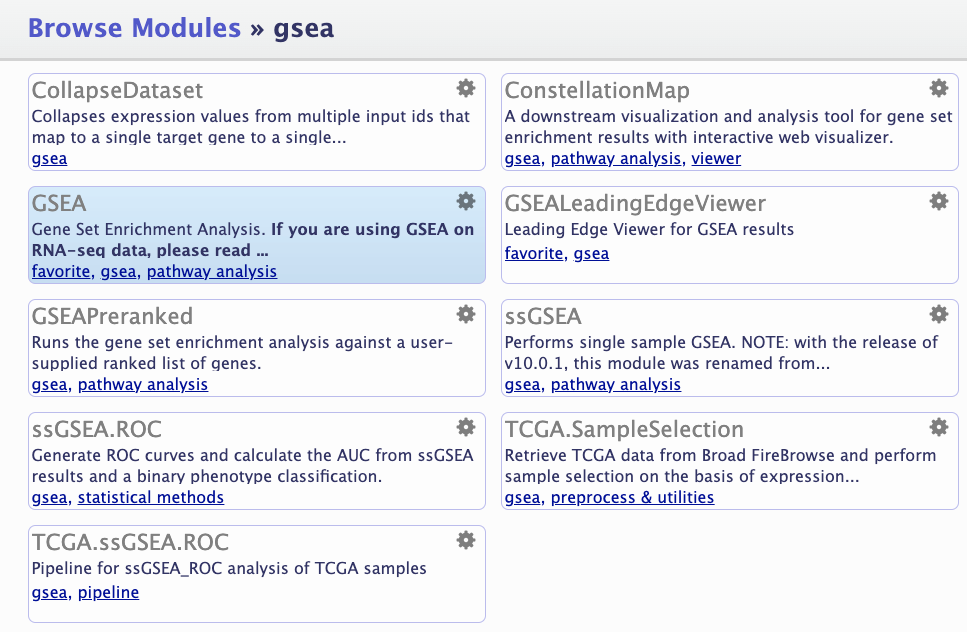
\includegraphics[width=1\linewidth]{images/Browse_Modules_gsea} 

}

\caption{Browse GSEA module in GenePattern}\label{fig:unnamed-chunk-24}
\end{figure}

\hypertarget{steps-to-perform-gsea}{%
\subsection{Steps to Perform GSEA:}\label{steps-to-perform-gsea}}

\begin{enumerate}
\def\labelenumi{\arabic{enumi}.}
\tightlist
\item
  Basic Parameters
\end{enumerate}

- Create both \texttt{.gct} and \texttt{.cls} files following \href{degust.html}{this scrit in R}

- Load the \texttt{.gct} input file in the \texttt{expression\ dataset} tab and \texttt{.cls} file in the \texttt{phenotype\ labels} tab

- Select a \texttt{.gmt} file (Gene Matrix Transposed) from the \texttt{gene\ sets\ database} tab

- Set permutation under \texttt{number\ of\ permutations} tab

- Type of the permuattaion to be set under \texttt{permutation\ type} tab

- Select an appropriate DNA Chip annotation file from \texttt{chip\ platform\ file} tab

- Name the output file in \texttt{output\ file\ name} tab

\begin{enumerate}
\def\labelenumi{\arabic{enumi}.}
\setcounter{enumi}{1}
\tightlist
\item
  Advanced Parameters
\end{enumerate}

- Scoring Scheme:

\begin{itemize}
\item
  K-S: The score increment is the same for all genes in \emph{S} regardless of their ranking or correlation strength.
\item
  WEighted: the score increment for each gene in \emph{S} is weighted by its correlation with the phenotype, typically the absolute value of the correlation or ranking metric.
\end{itemize}

- Metric for ranking genes: Ranking metric of interest can be chosen from drop down menu. A detailed description od the metrics is given on \href{https://docs.gsea-msigdb.org/\#GSEA/GSEA_User_Guide/\#metrics-for-ranking-genes}{GSEA-MSigDB Documentation}.

\begin{itemize}
\item
  Categorical Phenotypes: Signal-to-Noise Ratio, t-Test, Ratio of Classes, Log2 Ratio of Classes
\item
  Continuous Phenotypes: Pearson Correlation, Spearman Correlation
\end{itemize}

- Minimum and Maximum size of gene sets can be set using \texttt{max\ gene\ set\ size} and \texttt{min\ gene\ set\ size} tabs

\hypertarget{browse-the-gsea-results}{%
\subsubsection{Browse the GSEA results}\label{browse-the-gsea-results}}

Once the job has been queued and successfully run, the output will be listd on the left panel under \texttt{Jobs} tab:

\begin{figure}

{\centering 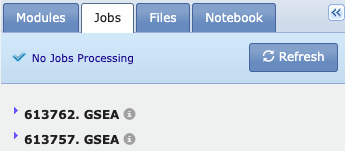
\includegraphics{images/GenePattern-Jobs} 

}

\caption{Job status in GenePattern}\label{fig:unnamed-chunk-25}
\end{figure}

Of the most important files is the \texttt{.zip} file that was earlier specified under \texttt{output\ file\ name} tab in Basic parameters section which includes all the results. The results can also be navigated using the single files listed under the job id.

For Pezzini experiment, two \texttt{html} files generated for each of up- and down-regulated gene sets, something like:

\begin{itemize}
\item
  gsea\_report\_for\_Diff\_1731388275794.html
\item
  gsea\_report\_for\_Nodiff\_1731388275794.html
\end{itemize}

The tabulated versions of the results are given in \texttt{.tsv} format:

\begin{itemize}
\item
  gsea\_report\_for\_Diff\_1731388275794.tsv
\item
  gsea\_report\_for\_Nodiff\_1731388275794.tsv
\end{itemize}

The GSEA result tables have the following header and below is given details of one gene set:

\begin{table}

\caption{\label{tab:unnamed-chunk-26}Summary of GSEA Results for REACTOME_FRS_MEDIATED_FGFR2_SIGNALING Gene Set}
\centering
\begin{tabular}[t]{l|l}
\hline
Parameter & Value\\
\hline
GS (follow link to MSigDB) & [REACTOME\_FRS\_MEDIATED\_FGFR2\_SIGNALING](https://www.gsea-msigdb.org/gsea/msigdb/human/geneset/REACTOME\_FRS\_MEDIATED\_FGFR2\_SIGNALING)\\
\hline
GS DETAILS & Details ...\\
\hline
SIZE & 16\\
\hline
ES & 0.83905387\\
\hline
NES & 1.7128055\\
\hline
NOM p-val & 0\\
\hline
FDR q-val & 0.03902518\\
\hline
FWER p-val & 0.648\\
\hline
RANK AT MAX & 995\\
\hline
LEADING EDGE & tags=38\%, list=7\%, signal=40\%\\
\hline
\end{tabular}
\end{table}

The leading edge column has three values:

\begin{itemize}
\tightlist
\item
  tags: 38\% of the genes in the gene set are key to the enrichment result.
\item
  list: These genes make up 7\% of the total gene list being analyzed.
\item
  signal: They contribute 40\% of the enrichment signal, highlighting their importance in driving the association between this gene set and the biological phenotype being studied.
\end{itemize}

\hypertarget{challenge-how-do-different-ranking-metrics-impact-the-output}{%
\subsubsection*{\texorpdfstring{\textbf{Challenge:} How do different ranking metrics impact the output?}{Challenge: How do different ranking metrics impact the output?}}\label{challenge-how-do-different-ranking-metrics-impact-the-output}}
\addcontentsline{toc}{subsubsection}{\textbf{Challenge:} How do different ranking metrics impact the output?}

Run GSEA analysis using Hallmark gene sets with two metrics (tTest and Ratio\_of\_Classes). What are the upregulated terms (FDR \textless{} 0.1) in the \texttt{Diff} class, based on the t-test and Ratio of Classes metrics?

\hypertarget{question-2}{%
\subsubsection*{\texorpdfstring{\textbf{Question }}{Question }}\label{question-2}}
\addcontentsline{toc}{subsubsection}{\textbf{Question }}

Why might the HALLMARK\_CHOLESTEROL\_HOMEOSTASIS gene set be upregulated specifically in the differentiation condition of SH-SY5Y cells in \href{https://pubmed.ncbi.nlm.nih.gov/27422411/}{Pezzini, et al 2016} experiment?

Show

\begin{itemize}
\tightlist
\item
  Relevance: Cholesterol is essential for neuronal function and membrane fluidity, particularly in processes like axonal growth and synapse formation. Neurons have a high demand for cholesterol, especially during differentiation when they extend axons and dendrites.
\item
  Possible Insight: Upregulation of genes in this set could signify that differentiating cells are actively producing or transporting cholesterol to support membrane synthesis and cellular remodeling required for mature neuronal structures.
\end{itemize}

\hypertarget{section-4}{%
\subsubsection*{}\label{section-4}}
\addcontentsline{toc}{subsubsection}{}

\hypertarget{fea-in-reactome}{%
\section{\texorpdfstring{FEA in Reactome }{FEA in Reactome }}\label{fea-in-reactome}}

Reactome is an open-source database of curated biological pathways across species, offering pathway maps and enrichment tools to analyse gene lists in a pathway-focused context. It's ideal for visualising data within established biochemical and cellular processes.

\hypertarget{steps-to-perform-ora-in-reactome}{%
\subsection{Steps to perform ORA in Reactome:}\label{steps-to-perform-ora-in-reactome}}

\begin{itemize}
\tightlist
\item
  Hit the \texttt{Analysis\ Tools} tab
\end{itemize}

\begin{figure}

{\centering 
\includegraphics[width=1\linewidth]{images/reactome-tabs} 

}

\caption{Analysis in Reactome}\label{fig:unnamed-chunk-27}
\end{figure}

\begin{itemize}
\tightlist
\item
  Choose \texttt{Analyse\ gene\ list} from the left panel
\end{itemize}

\begin{figure}

{\centering 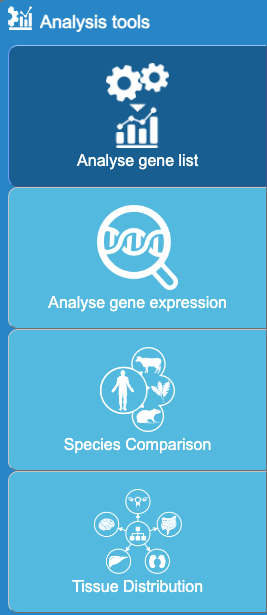
\includegraphics[width=0.2\linewidth]{images/reactome-analysis-tools} 

}

\caption{Analysis Tools in Reactome}\label{fig:unnamed-chunk-28}
\end{figure}

\begin{itemize}
\item
  Upload list of features on the box or choose a file, hit continue
\item
  Select prefered options:

  - Project to Human: This option will convert identifiers from non-human species into human equivalents, allowing you to analyse data across species.

  - Include interactors: This option integrates interactors from IntAct, a protein interaction database. Including interactors broadens the background network, potentially offering deeper insights.
\item
  Hit Analyse!
\end{itemize}

\hypertarget{steps-to-perform-gsa-in-reactome}{%
\subsection{Steps to perform GSA in Reactome:}\label{steps-to-perform-gsa-in-reactome}}

\begin{itemize}
\tightlist
\item
  If \texttt{Analyse\ gene\ expression} was chosen instead, Reactome offers the following gene set analysis:
\end{itemize}

\begin{figure}

{\centering 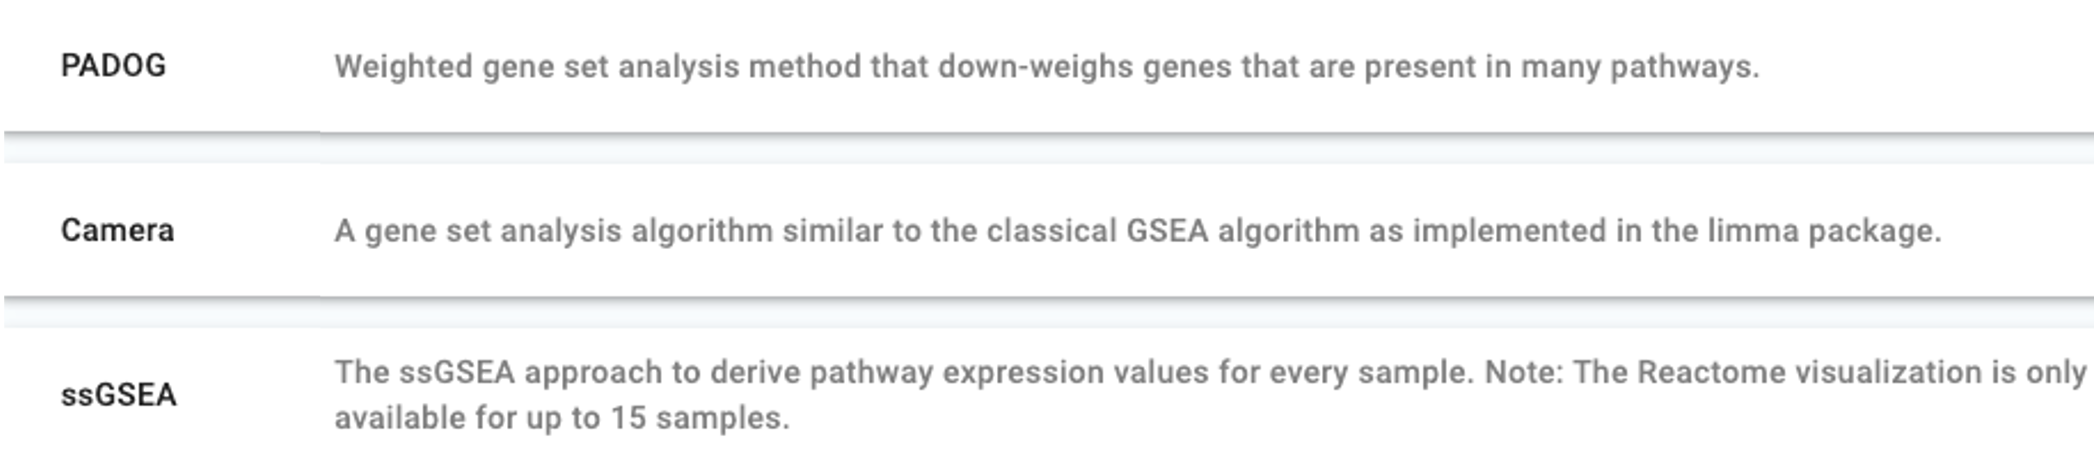
\includegraphics[width=1\linewidth]{images/reactome-gsea-methods} 

}

\caption{Ractome GSA }\label{fig:unnamed-chunk-29}
\end{figure}

\begin{itemize}
\item
  Lets try CAMERA as it represents the \texttt{camera()} function of \texttt{limma} package in \texttt{R} for a gene set analysis.
\item
  Choose TMM normalisation to ensure consistency with the input data used in other tools within our workshop.
\item
  Select data type and provide input data
\end{itemize}

\begin{figure}

{\centering 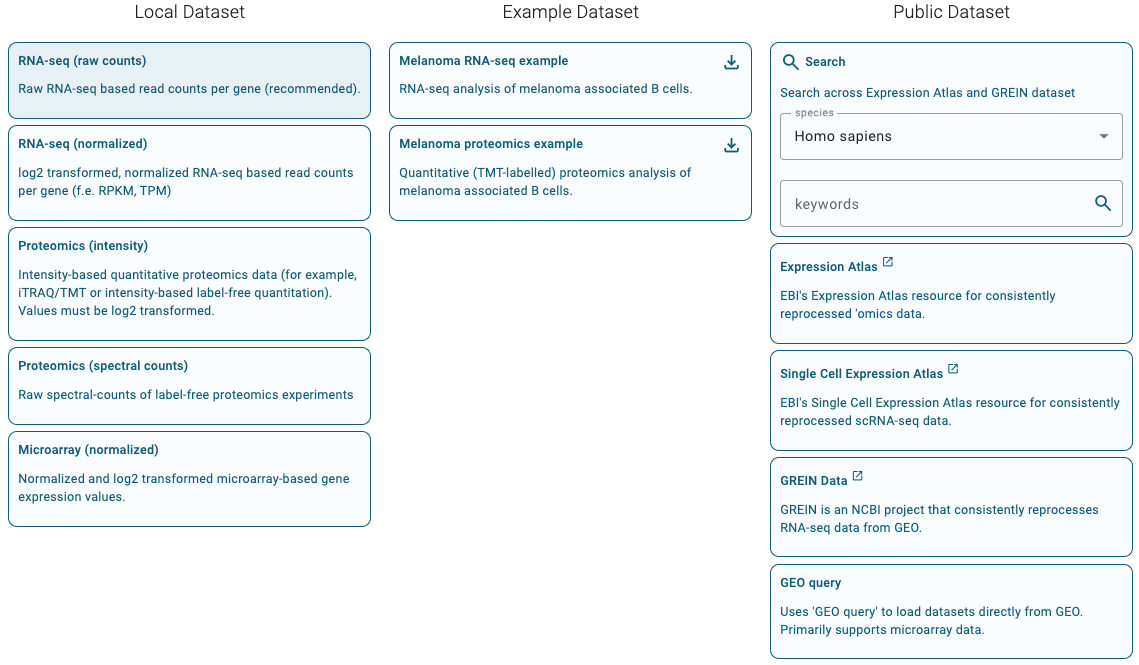
\includegraphics[width=1\linewidth]{images/reactome-gsea-select-data} 

}

\caption{Ractome GSA - data type}\label{fig:unnamed-chunk-30}
\end{figure}

\begin{itemize}
\tightlist
\item
  Annotate columns by adding extra info as follows:
\end{itemize}

\begin{figure}

{\centering 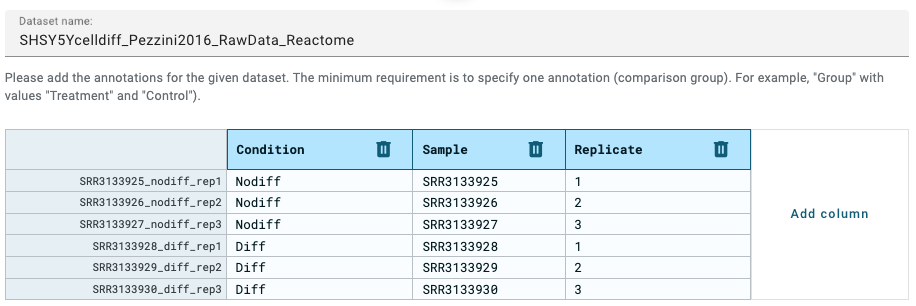
\includegraphics[width=1\linewidth]{images/reactome-gsea-add-column} 

}

\caption{Pathway diagram }\label{fig:unnamed-chunk-31}
\end{figure}

\begin{itemize}
\item
  Save dataset and Continue
\item
  You can now browse the results
\end{itemize}

\hypertarget{browse-the-reactome-results}{%
\subsection{Browse the Reactome results}\label{browse-the-reactome-results}}

Results can be interactively browsed using the reactome pathway or voronoi visualisation modes:

User can explore the pathway names listed in the table within the \texttt{Analysis} tab and they are displayed as popups on the pathway diagrams.

One can also select a pathway of interest by navigating through the left panel or by simply searching for the term in the search box.

The enriched table can be downloaded as shown below:

\begin{figure}

{\centering 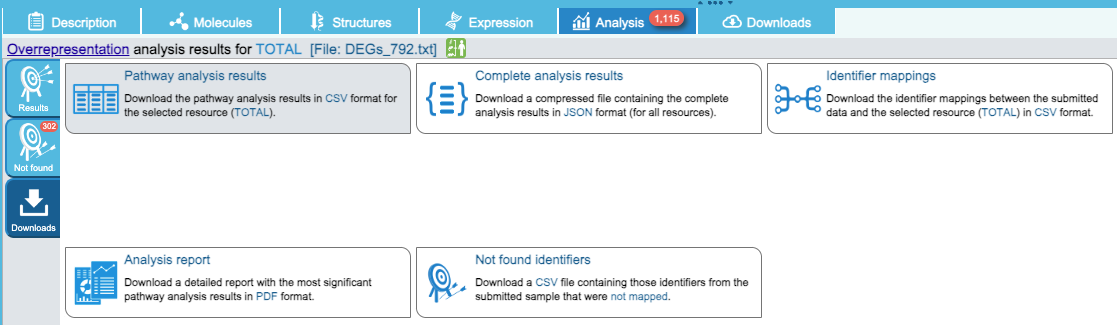
\includegraphics[width=1\linewidth]{images/reactome-download-table} 

}

\caption{Table of ORA with Reactome}\label{fig:unnamed-chunk-32}
\end{figure}

The diagram can be downloaded using this icons:

Here is a sample pathway diagram from Reactome GSA.

\begin{figure}

{\centering 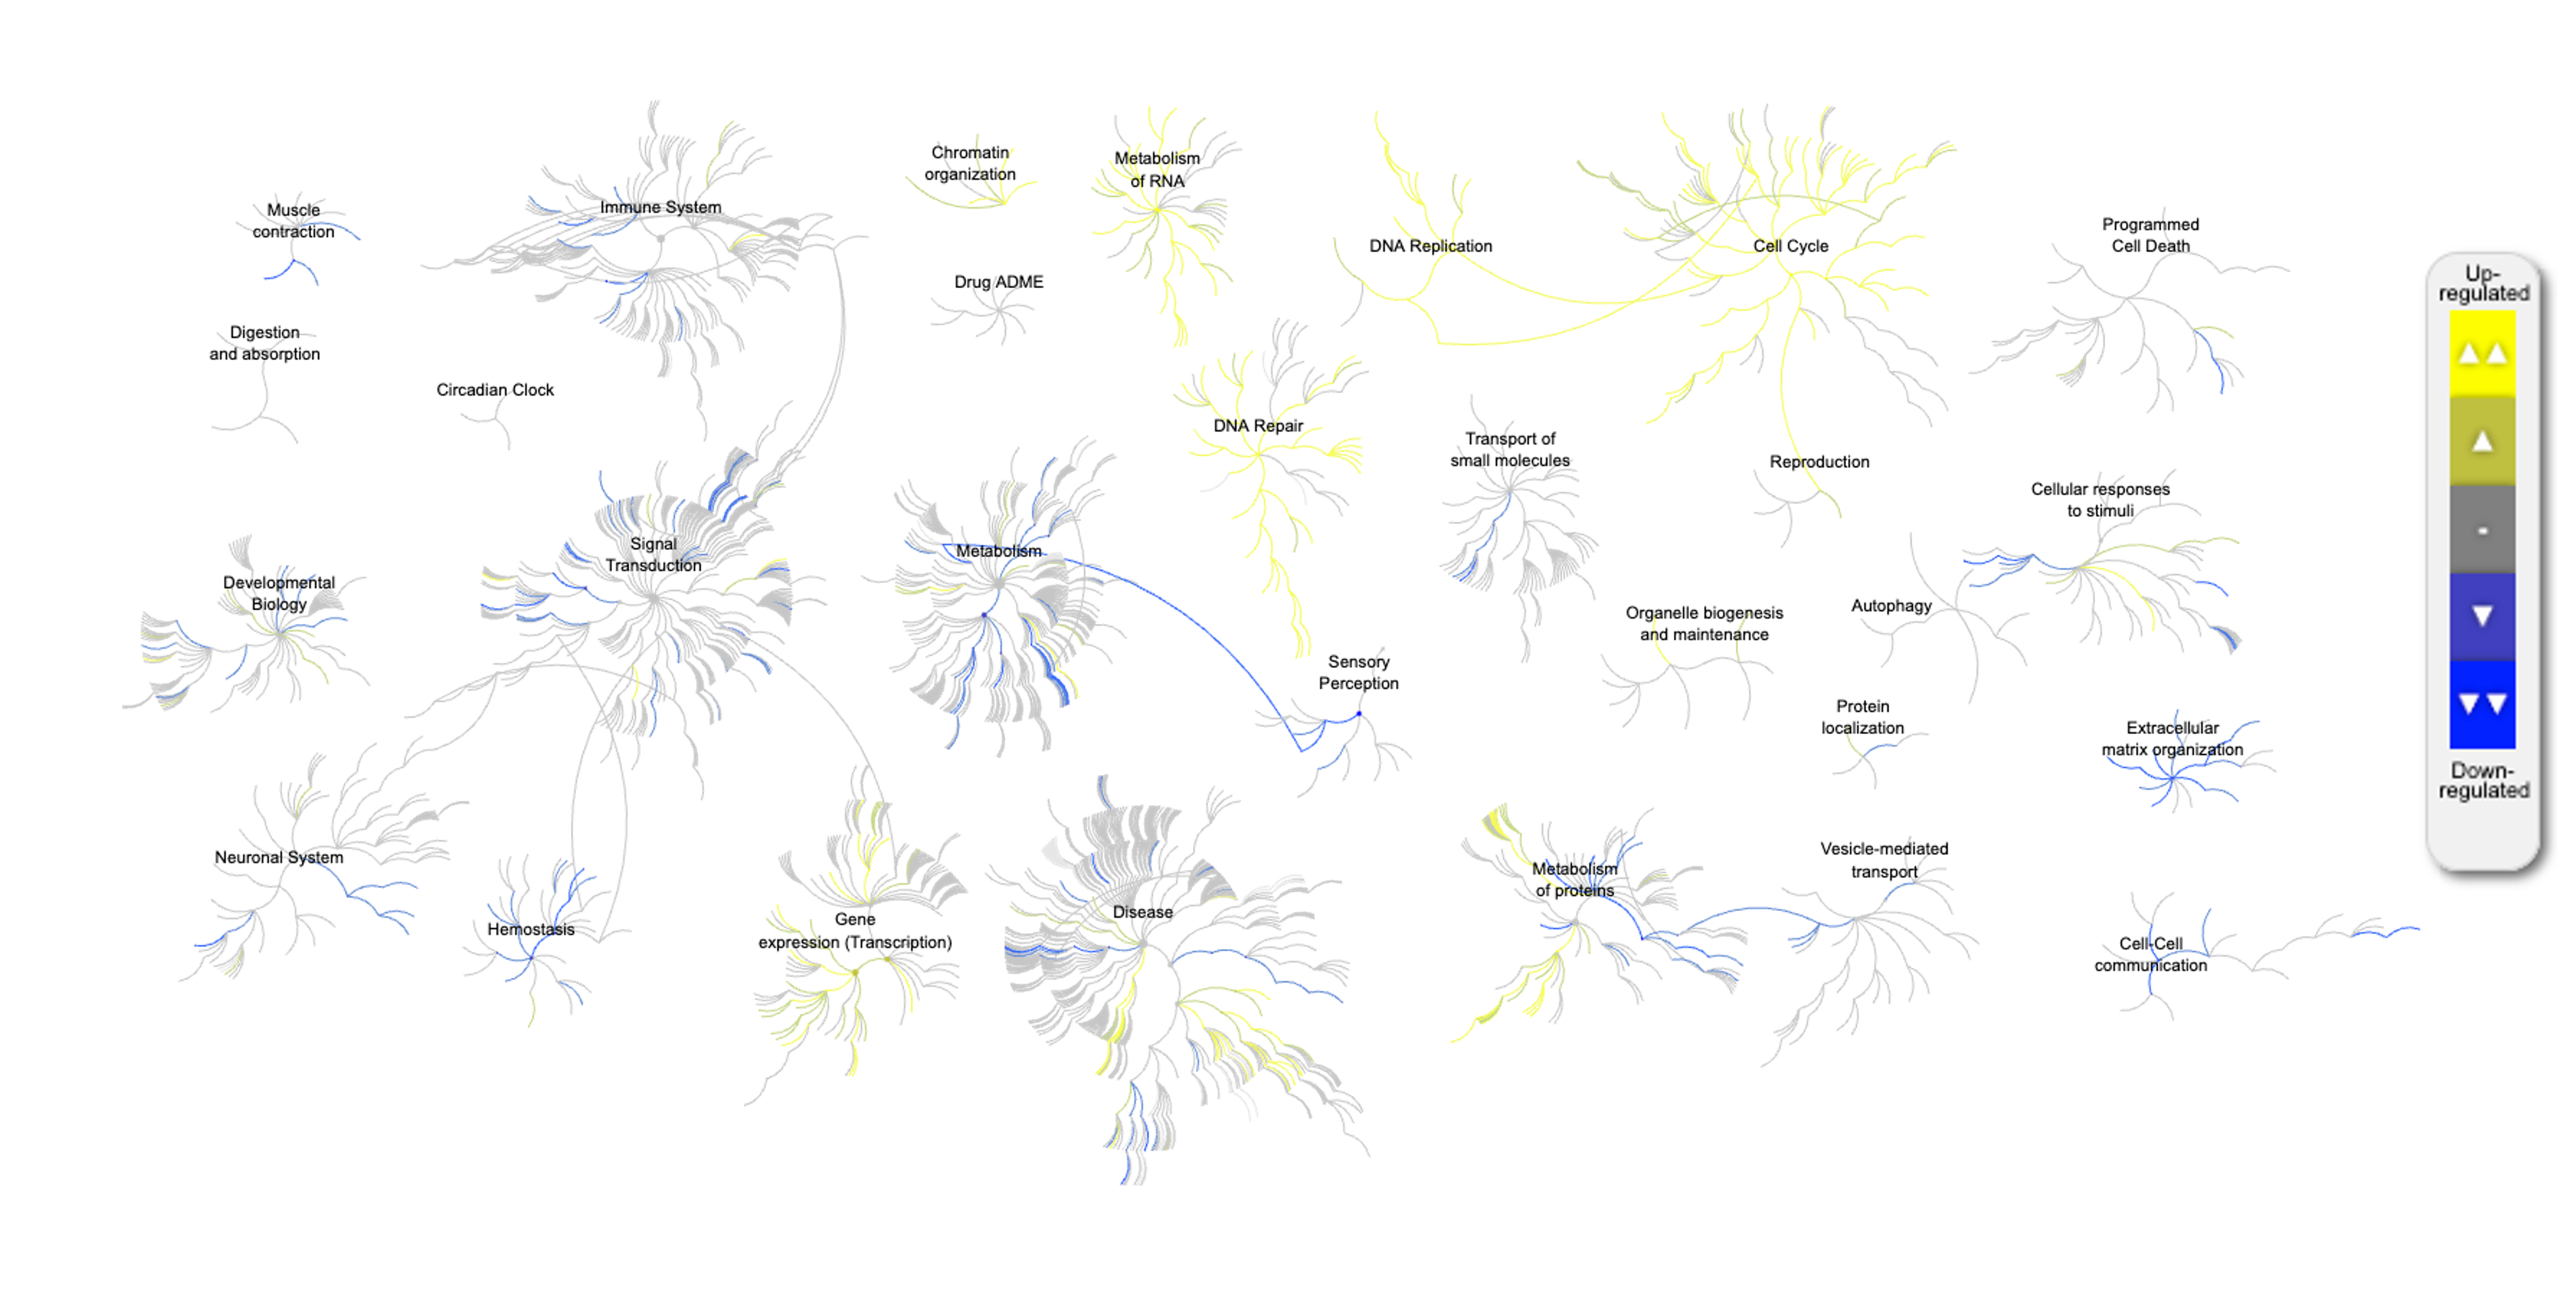
\includegraphics[width=1\linewidth]{images/reactome-PathwaysOverview-expression-data} 

}

\caption{Pathway diagram - GSA}\label{fig:unnamed-chunk-33}
\end{figure}

In case \texttt{ssGSEA} was selected, an overall output would look like below:

\begin{figure}

{\centering 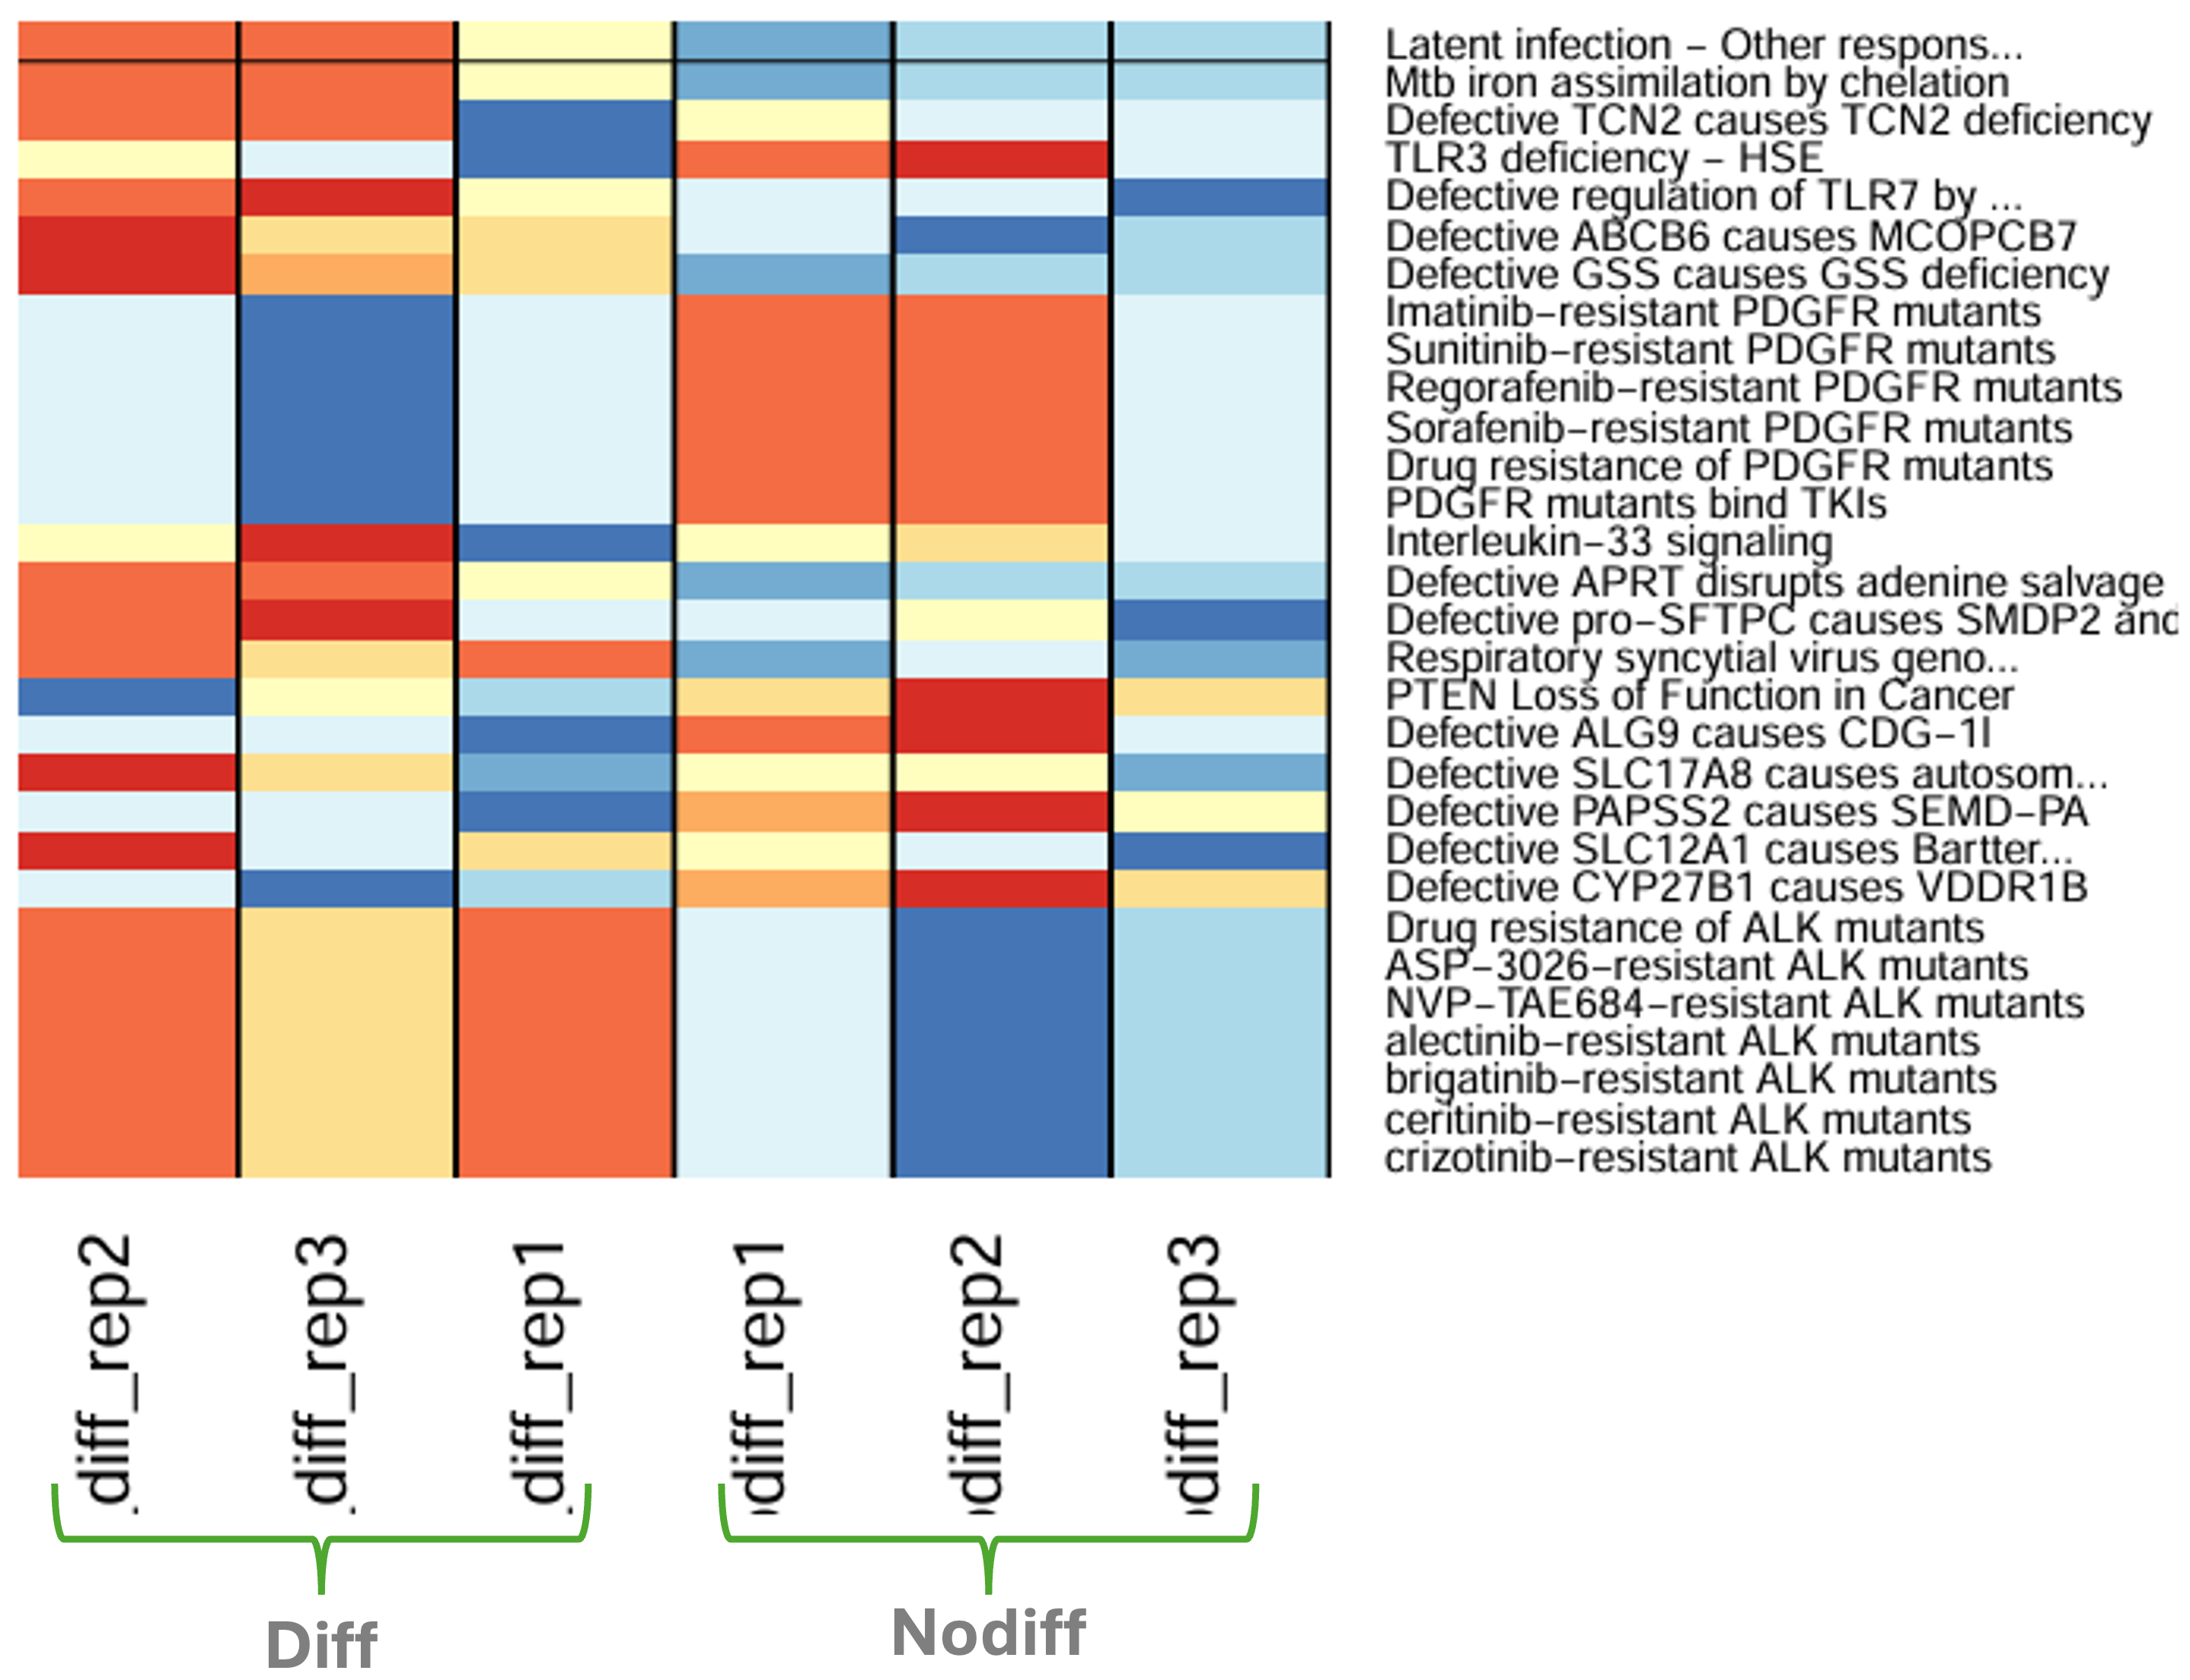
\includegraphics[width=0.7\linewidth]{images/reactome-ssGSEA} 

}

\caption{Expression of top 30 pathways with ssGSEA}\label{fig:unnamed-chunk-34}
\end{figure}

\hypertarget{section-5}{%
\subsubsection*{}\label{section-5}}
\addcontentsline{toc}{subsubsection}{}

\hypertarget{question-3}{%
\subsubsection*{\texorpdfstring{\textbf{Question }}{Question }}\label{question-3}}
\addcontentsline{toc}{subsubsection}{\textbf{Question }}

When running FEA in Reactome, how do you prefer the analysis methods?

- PADOG (Pathway Analysis with Down-weighting of Overlapping Genes)

- CAMERA (Correlation Adjusted Mean Rank)

- ssGSEA (Single Sample Gene Set Enrichment Analysis)

\hypertarget{section-6}{%
\subsubsection*{}\label{section-6}}
\addcontentsline{toc}{subsubsection}{}

\hypertarget{reporting-results}{%
\chapter{Reporting results}\label{reporting-results}}

Once we have done an enrichment analysis - how to communicate the results? Like everything - it depends what you need to say. Some examples are below.

\hypertarget{in-text}{%
\section{In text}\label{in-text}}

If you just need to emphasise that the differential expression relates to a condition of interest, you don't need much:

\begin{quote}
Genes differentially expressed after SH-SY5Y cell differentiation were enriched for GO term ``regulation of neurogenesis'', adjusted pval \textless{} 0.01).
\end{quote}

And in the methods:

\begin{quote}
Enrichment calculated for differentially expressed genes with the g:GOSt enrichment tool \href{https://academic.oup.com/nar/article/47/W1/W191/5486750}{(Raudvere et al, 2019)} using a background of tested genes.
\end{quote}

\hypertarget{as-a-table}{%
\section{As a table}\label{as-a-table}}

For a more complete view, a table of the significant or top \emph{n} terms can be useful. E.g In a supplementary figure

The top 10 enriched GO terms for the differentially expressed genes;

\begin{longtable}[]{@{}
  >{\raggedright\arraybackslash}p{(\columnwidth - 8\tabcolsep) * \real{0.4118}}
  >{\raggedright\arraybackslash}p{(\columnwidth - 8\tabcolsep) * \real{0.1176}}
  >{\raggedleft\arraybackslash}p{(\columnwidth - 8\tabcolsep) * \real{0.1765}}
  >{\raggedleft\arraybackslash}p{(\columnwidth - 8\tabcolsep) * \real{0.1078}}
  >{\raggedleft\arraybackslash}p{(\columnwidth - 8\tabcolsep) * \real{0.1863}}@{}}
\toprule\noalign{}
\begin{minipage}[b]{\linewidth}\raggedright
\url{GO:BP} Term
\end{minipage} & \begin{minipage}[b]{\linewidth}\raggedright
Term ID
\end{minipage} & \begin{minipage}[b]{\linewidth}\raggedleft
Adjusted p-value
\end{minipage} & \begin{minipage}[b]{\linewidth}\raggedleft
Term Size
\end{minipage} & \begin{minipage}[b]{\linewidth}\raggedleft
Num DE Genes
\end{minipage} \\
\midrule\noalign{}
\endhead
\bottomrule\noalign{}
\endlastfoot
system process & \url{GO:0003008} & 2.90E-04 & 1243 & 45 \\
nervous system development & \url{GO:0007399} & 4.19E-04 & 1985 & 60 \\
regulation of cell development & \url{GO:0060284} & 1.98E-03 & 795 & 33 \\
central nervous system development & \url{GO:0007417} & 2.67E-03 & 805 & 33 \\
regulation of neurogenesis & \url{GO:0050767} & 5.59E-03 & 707 & 30 \\
regulation of nervous system development & \url{GO:0051960} & 5.78E-03 & 790 & 32 \\
regulation of cell differentiation & \url{GO:0045595} & 6.03E-03 & 1471 & 47 \\
multicellular organismal process & \url{GO:0032501} & 2.04E-02 & 5300 & 111 \\
system development & \url{GO:0048731} & 2.88E-02 & 3668 & 85 \\
neurogenesis & \url{GO:0022008} & 4.36E-02 & 1375 & 43 \\
\end{longtable}

\hypertarget{as-a-figure}{%
\section{As a figure}\label{as-a-figure}}

Plots of -log p-value are a popular option for a figure. By taking the exponent of the p-value bigger bars indicate more significance.

For instance, this figure is taken from the \href{https://link.springer.com/article/10.1007\%2Fs10571-016-0403-y}{(Pezzini et al.~2017)} paper.
Note that in this figure shows 2 specifics categories from the IPA (ingenuity) database using the IPA tool (not covered here), so the terms themselves differ.

\includegraphics{https://monashbioinformaticsplatform.github.io/enrichment_analysis_workshop/img/NegLogPvalPlot_Pezzini2017.png}

You can also build on such a plot with number of genes and the like. For an example, see the `bubble' chart produced by a package called pathfindR here: \url{https://www.biostars.org/p/322415/}

\begin{center}\rule{0.5\linewidth}{0.5pt}\end{center}

There are also tools like cluego (a cytoscape plugin) that build enriched terms into a network : \url{http://apps.cytoscape.org/apps/cluego}

\hypertarget{resources}{%
\chapter{Resources}\label{resources}}

The following tools might be useful for downstream functional analysis; this includes some not covered in todays workshop.

Note that most of these tools do more than just enrichment tests, and some include their own databases.

\hypertarget{gprofiler-ggost}{%
\section{g:Profiler / g:GOSt}\label{gprofiler-ggost}}

\url{https://biit.cs.ut.ee/gprofiler/gost}

The g:GOSt `functional profiling' tool of g:Profiler calculates
It has a clean modern interface and a handy summary of which genes contribute to the enrichment.

\begin{figure}
\includegraphics[width=1\linewidth]{https://monashbioinformaticsplatform.github.io/enrichment_analysis_workshop/img/gprofiler} \caption{The gProfiler front page}\label{fig:unnamed-chunk-37}
\end{figure}

\hypertarget{panther}{%
\section{PANTHER}\label{panther}}

\url{http://www.pantherdb.org/}

PANTHER performs overrepresentation tests across multiple databases; Gene ontology, reactome, PANTHER pathways and protein classes. Allows more control over the statistical test used and clearly summarises what was actually done.

\begin{figure}
\includegraphics[width=1\linewidth]{https://monashbioinformaticsplatform.github.io/enrichment_analysis_workshop/img/panther} \caption{PANTHER}\label{fig:unnamed-chunk-38}
\end{figure}

\hypertarget{david}{%
\section{DAVID}\label{david}}

\url{https://david.ncifcrf.gov/}

Via its `functional annotation' tool, DAVID allows you to calculate functional enrichment across a number of databases ; Gene Ontology, KEGG, reactome and others. Reliable, with a slightly clunky interface.

\begin{figure}
\includegraphics[width=1\linewidth]{https://monashbioinformaticsplatform.github.io/enrichment_analysis_workshop/img/david} \caption{DAVID}\label{fig:unnamed-chunk-39}
\end{figure}

\hypertarget{enrichr}{%
\section{Enrichr}\label{enrichr}}

\url{https://amp.pharm.mssm.edu/Enrichr/}

Enrichr easily calculates enrichment across a wide range of databases. Currently does not allow for a background set.

\begin{figure}
\includegraphics[width=1\linewidth]{https://monashbioinformaticsplatform.github.io/enrichment_analysis_workshop/img/enrichr} \caption{Enrichr}\label{fig:unnamed-chunk-40}
\end{figure}

\hypertarget{reactome-1}{%
\section{Reactome}\label{reactome-1}}

\url{https://reactome.org/}

The core of reactome is the reactome pathways and browser. ALthough other tools use the reactome database, the reactome website provides a means to browse enrichment within the pathway browser view.

\begin{figure}
\includegraphics[width=1\linewidth]{https://monashbioinformaticsplatform.github.io/enrichment_analysis_workshop/img/reactome} \caption{Reactome}\label{fig:unnamed-chunk-41}
\end{figure}

\hypertarget{biocyc}{%
\section{Biocyc}\label{biocyc}}

\url{https://biocyc.org/}

Biocyc is another suite of tools for enrichment and pathway browsing, which is particularly useful for prokaryotic work. It is licensed, but Monash does have a license.

\begin{figure}
\includegraphics[width=1\linewidth]{https://monashbioinformaticsplatform.github.io/enrichment_analysis_workshop/img/biocyc} \caption{Biocyc}\label{fig:unnamed-chunk-42}
\end{figure}

\hypertarget{string}{%
\section{STRING}\label{string}}

\url{https://string-db.org/}

STRING is not a functional enrichment tool, rather it is a convenient way to explore interactions within a genelist. Results are viewed as an interaction network. Best suited to smaller genelists.

\begin{figure}
\includegraphics[width=1\linewidth]{https://monashbioinformaticsplatform.github.io/enrichment_analysis_workshop/img/string} \caption{STRING}\label{fig:unnamed-chunk-43}
\end{figure}

\hypertarget{gene-ontology}{%
\section{Gene Ontology}\label{gene-ontology}}

\url{http://geneontology.org/}

Gene Ontology (GO) terms are the most widely use set of functional annotations, used by many enrichment tools. The gene ontology resource website itself provides several tools for browsing the GO term hierarchy.

\begin{figure}
\includegraphics[width=1\linewidth]{https://monashbioinformaticsplatform.github.io/enrichment_analysis_workshop/img/go} \caption{Gene Ontology}\label{fig:unnamed-chunk-44}
\end{figure}

\hypertarget{kegg}{%
\section{KEGG}\label{kegg}}

\url{https://www.genome.jp/kegg/}

A well known curated pathway database. It is used by many other tools but with a caveat - KEGG moved to a subscription model in 2011, and so enrichment tools need to use the last open release from 2011. However up to date KEGG pathways are browsable directly through their website.

\begin{figure}
\includegraphics[width=1\linewidth]{https://monashbioinformaticsplatform.github.io/enrichment_analysis_workshop/img/kegg} \caption{KEGG}\label{fig:unnamed-chunk-45}
\end{figure}

\hypertarget{gsea-and-msigdb}{%
\section{GSEA and MSigDB}\label{gsea-and-msigdb}}

\url{http://software.broadinstitute.org/gsea/index.jsp}

The desktop-based GSEA tool is (one of many) gene set enrichment approaches. It uses of gene rankings across all genes rather than hypogeometric or fishers-exact tests of genelist enrichment. MSigDB (Molecular signatures database) is a suite of annotation databases suitable for GSEA analysis.

\begin{figure}
\includegraphics[width=1\linewidth]{https://monashbioinformaticsplatform.github.io/enrichment_analysis_workshop/img/gsea} \caption{MSigDB}\label{fig:unnamed-chunk-46}
\end{figure}

\hypertarget{metaboanalyst}{%
\section{MetaboAnalyst}\label{metaboanalyst}}

MetaboAnalyst is popular among the metabolomics community for statistical, functional and integrative analysis of metabolomics data. It has a feature called \textbf{Functional enrichment analysis}, which performs metabolite set enrichment analysis, metabolic pathway analysis, and pathway activity prediction from MS peaks.

\begin{figure}
\includegraphics[width=1\linewidth]{https://monashbioinformaticsplatform.github.io/enrichment_analysis_workshop/img/metaboanalyst} \caption{MetaboAnalyst}\label{fig:unnamed-chunk-47}
\end{figure}

\hypertarget{cytoscape}{%
\section{Cytoscape}\label{cytoscape}}

\url{https://cytoscape.org/}

Cytoscape is a desktop-based biological network analysis / visualization tool, rather than a functional enrichment tool (although plugins can change that). It is mentioned here because it is often useful as a next step when you need to create custom figures showing the interactions of an interesting biological pathway.

\begin{figure}
\includegraphics[width=1\linewidth]{https://monashbioinformaticsplatform.github.io/enrichment_analysis_workshop/img/cytoscape} \caption{Cytoscape}\label{fig:unnamed-chunk-48}
\end{figure}

\hypertarget{part-day-2}{%
\chapter{(PART) Day 2}\label{part-day-2}}

\hypertarget{r-environment-set-up}{%
\chapter{R environment set up}\label{r-environment-set-up}}

For today's session, we will be using the \href{https://www.r-project.org/}{R} statistical programming language to perform functional enrichmemt analysis using a range of dedicated R packages. To simplify our work, we will be using the \href{https://posit.co/download/rstudio-desktop/}{RStudio} integrated development environment.

This will create a central place to write code, comments, run code, view and save graphics.


\includegraphics{images/rstudio_logo.png}

~

\hypertarget{rstudio-basics}{%
\section{RStudio basics}\label{rstudio-basics}}

RStudio with all the required R packages for today's activities are installed on your VM.

➤ Open the RStudio VM using the credentials provided to you.

\begin{itemize}
\tightlist
\item
  \textbf{TBA:} - ensure that they have the VM details by now, if not provide further instructions within this section
\end{itemize}

When RStudio opens, you will see empty \texttt{Console}, \texttt{History} and \texttt{Plots} panes.

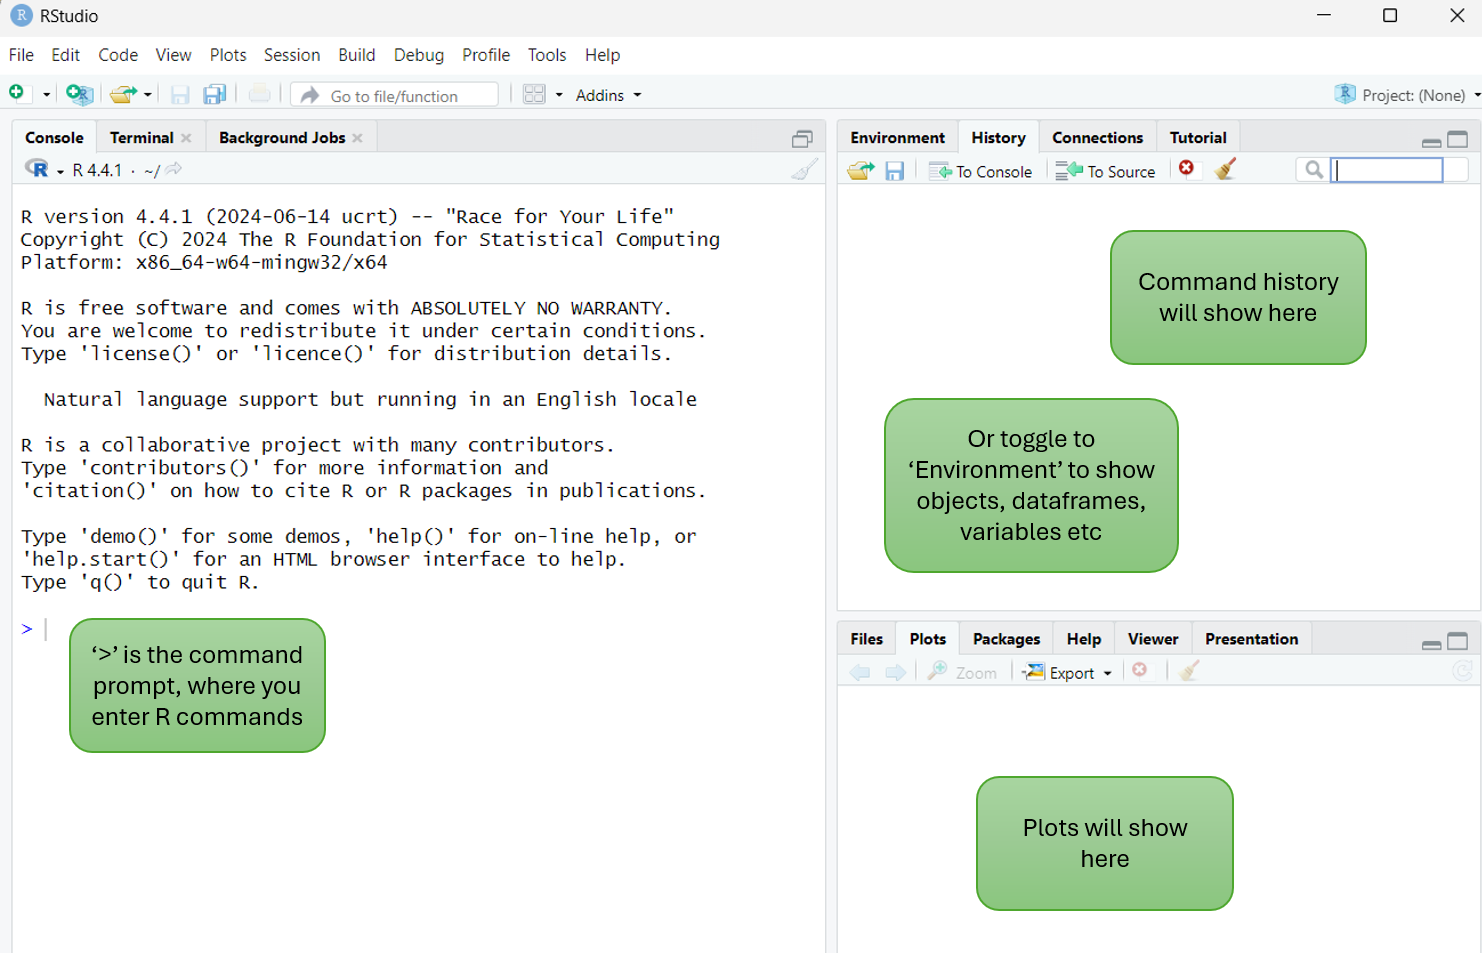
\includegraphics[width=1\textwidth,height=\textheight]{images/rstudio-default-open.png}

~

You can toggle to other panes, for example change \texttt{Console} to \texttt{Terminal} or change \texttt{Plots} to \texttt{Files}.

:file\_folder: Since your VM only runs RStudio, you will use the \texttt{Files} pane to navigate your workshop folder and view any output files we generate.

The \texttt{Console} contains the command prompt (\texttt{\textgreater{}}) which is where R commands are entered.

~

➤ Test this out by copy pasting or typing the below command into your console then pressing \texttt{enter} key. This will print the path of your current working directory:

\begin{Shaded}
\begin{Highlighting}[]
\FunctionTok{getwd}\NormalTok{()}
\end{Highlighting}
\end{Shaded}

Your path will be something like \texttt{/home/user1}.

If you are unfamiliar with R, don't worry because we will provide all the R code that you need to complete today's workshop :smiley:

~

➤ Click on \texttt{Environment} to change the pane to list all active objects in your R session.

An object refers to things like imported datasets, R dataframes, variables, etc. For a new session, the environment is empty.

~

Let's put something in there:

➤ Create an R variable called \texttt{name} and fill it with your name, then print it with the \texttt{cat} command:

\begin{Shaded}
\begin{Highlighting}[]
\NormalTok{name }\OtherTok{\textless{}{-}} \StringTok{\textquotesingle{}Cali\textquotesingle{}}
\FunctionTok{cat}\NormalTok{(name)}
\end{Highlighting}
\end{Shaded}

Note that the object \texttt{name} is now listed in the environment.

~

Now let's see the \texttt{plots} pane in action by creating a simple dummy barplot:

➤ Copy paste the below code into your console then press enter:

\begin{Shaded}
\begin{Highlighting}[]
\NormalTok{values }\OtherTok{\textless{}{-}} \FunctionTok{c}\NormalTok{(}\DecValTok{5}\NormalTok{, }\DecValTok{10}\NormalTok{, }\DecValTok{15}\NormalTok{)}
\NormalTok{labels }\OtherTok{\textless{}{-}} \FunctionTok{c}\NormalTok{(}\StringTok{"A"}\NormalTok{, }\StringTok{"B"}\NormalTok{, }\StringTok{"C"}\NormalTok{)}
\FunctionTok{barplot}\NormalTok{(values, }\AttributeTok{names.arg =}\NormalTok{ labels)}
\end{Highlighting}
\end{Shaded}

You will now see a barplot in the \texttt{plots} pane, as well as 2 new objects in the \texttt{environment}. Note that the environment list also tells you what type of objects it is: for our \texttt{name} object, the double quotes indicate it's a single string, where \texttt{chr\ {[}1:3{]}} for \texttt{labels} shows that it is a \texttt{character\ vector} with 3 text elements. \texttt{num\ {[}1:3{]}} indicates that \texttt{values} is a numeric vector with 3 values. The takeaway message here is that the environment shows your active R objects, and that these are of different types. This is important to be aware of when working in R, because different packages and functions require different input types. During the workshop, we may need to convert our input to a \texttt{dataframe} or \texttt{vector} for example.

~

\hypertarget{download-input-data}{%
\section{Download input data}\label{download-input-data}}

\begin{itemize}
\tightlist
\item
  \textbf{TBA} - add link to zip file that has the input data and R notebooks for day2.
\end{itemize}

~

\hypertarget{r-notebooks}{%
\section{R notebooks}\label{r-notebooks}}

Today we will not be entering R commands directly into the console like this. We will instead be using an R notebook.

Using notebooks in RStudio is a great way to save your code and comments, as well as have the code output display inside the notebook. Notebooks can be easily shared with others so they can run your analysis, and also rendered to HTML which is a neat way of saving and presenting results to others.

➤ Open a new R notebook from the RStudio toolbar by selecting \texttt{File} → \texttt{New\ file} → \texttt{R\ Notebook}:

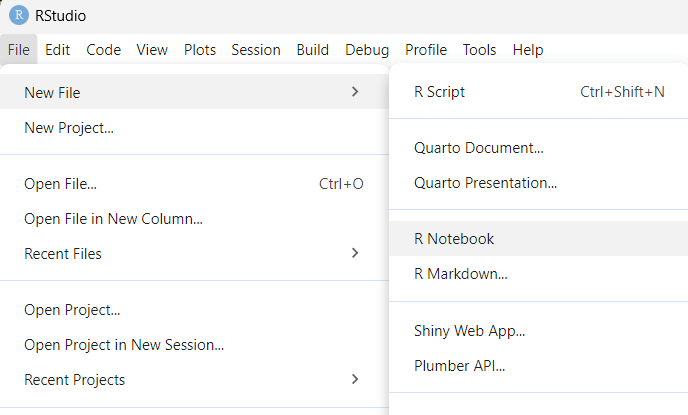
\includegraphics[width=1\textwidth,height=\textheight]{images/rstudio-new-notebook.png}

The new notebook opens in the \texttt{Editor} pane. It has a placeholder title and basic starting instructions.

~

\hypertarget{code-chunks}{%
\subsection{Code chunks}\label{code-chunks}}

A code chunk is placed within triple backticks (``\texttt{),\ and\ the\ language\ of\ the\ code\ is\ included\ on\ the\ first\ line,\ in\ this\ case}`r'`. Having code in chunks is a way of grouping and running related lines of code together.

Code chunks can be run by using the green arrow to the right of the chunk or by clicking inside the chunk and entering \texttt{ctrl\ +\ shift\ +\ enter}. There are additional run options under the \texttt{Run} menu from the top bar, for example \texttt{Run\ current\ chunk}, \texttt{Run\ next\ chunk}, or \texttt{Run\ all\ chunks\ below}.

Code chunks can also be given labels, by placing these inside the curly brackets, leaving a space after the \texttt{\textquotesingle{}r\textquotesingle{}}. Labels must be unique or rendering to HTML will fail with a message to correct the duplicated labels.

New code chunks can be added with the shortcut \texttt{ctrl\ +\ alt\ +\ i} or via the toolbar \texttt{Code} → \texttt{Insert\ chunk}.

~

➤ Run the demo code chunk that was included in the new notebook to plot \texttt{cars}

Note that the plot dispalys \emph{inside} the notebook, rather than within the plot pane as we saw earlier.

~

➤ Add a new code chunk by entering \texttt{ctrl\ +\ alt\ +\ i} and label it \texttt{barplot}. Then copy the dummy barplot code from earlier into the code chunk and run it

\begin{Shaded}
\begin{Highlighting}[]
\NormalTok{values }\OtherTok{\textless{}{-}} \FunctionTok{c}\NormalTok{(}\DecValTok{5}\NormalTok{, }\DecValTok{10}\NormalTok{, }\DecValTok{15}\NormalTok{)}
\NormalTok{labels }\OtherTok{\textless{}{-}} \FunctionTok{c}\NormalTok{(}\StringTok{"A"}\NormalTok{, }\StringTok{"B"}\NormalTok{, }\StringTok{"C"}\NormalTok{)}
\FunctionTok{barplot}\NormalTok{(values, }\AttributeTok{names.arg =}\NormalTok{ labels)}
\end{Highlighting}
\end{Shaded}

~

\hypertarget{rendered-html-notebooks}{%
\subsection{Rendered HTML notebooks}\label{rendered-html-notebooks}}

Next we will look at what a HTML version of the notebook looks like. In order to preview the HTML, we first need to save the notebook.

➤ Change the title to something of your choice and make any other edits you want to, such as deleting some of the default content

\textbf{Note:} don't delete the \texttt{output:\ html\_notebook} content from under the title! This will prevent the option to preview the html.

~

➤ Save the notebook (either \texttt{ctrl\ +\ s} or \texttt{File} → \texttt{Save\ as}) then preview the HTML by selecting \texttt{Preview} from the editor pane toolbar

\texttt{Preview} is for a quick check of how your notebook renders while working on it. For a fullly rendered, static document, use the \texttt{knit} function.

~

➤ Knit the notebook to HTML by selecting \texttt{Knit} → \texttt{Knit\ to\ HTML} from the editor pane toolbar

Note that the HTML is saved to your current working directory, which we previously verified was \texttt{/home/userN}. Check that the file appears where you expect it to via the \texttt{Files} pane (lower right).

For today's activities, you have downloaded and unzipped a folder containing the R notebooks required to run the analyses. After each activity, you may choose to knit the notebook to HTML to have a static record of your work :open\_book:

~

\hypertarget{a-fresh-workspace}{%
\subsection{A fresh workspace}\label{a-fresh-workspace}}

Next we will open the R notebook for the first analysis activity. It's ideal to start a new analysis with a clear environment, to avoid unintended object name clashes.

➤ Clear your environment by selecting \texttt{Session} → \texttt{Quit\ session} → \texttt{Dont\ save} →\texttt{Start\ mew\ session}

\textbf{Note:} when asked \texttt{Save\ workspace\ image\ to\ \textasciitilde{}/R.Data?} it is typically advisable to select \texttt{Don\textquotesingle{}t\ Save}. Not saving the workspace image can help avoid workspace clashes that are hard to resolve. You don't need to worry about losing data - after all, your input data is saved elsewhere, and your R code that produces all required outputs is safely saved within the notebook.

Saving the workspace image saves all objects from the session such as your variables and dataframes. This can save time if you need to close an analysis part way through and continue later. However, this can have drawbacks such as the clashes as mentioned, as well as large file size, relic objects cluttering thr workspace, old objects conflicting with new ones, etc. Since we will be performing discrete analysis tasks today, and not continuing on a growing body of work, selecting \texttt{Dont\ save} will be the most appropraite.

~

\hypertarget{working-directory}{%
\subsection{Working directory}\label{working-directory}}

Now that we have a clear workspace, we will prepare for the first analysis activity by opening the notebook and checking our working directory.

You have previosuly downloaded \texttt{Functional\_enrichment\_workshop\_2024}. This contains a folder \texttt{day\_2}.

➤ On the \texttt{Files} pane, open the \texttt{day\_2} folder and confirm that it contains the input data file \texttt{Pezzini\_DE.txt}

This will be our input file for the first activity.

~

➤ Load the notebook \texttt{Functional\_enrichment\_workshop\_2024/day\_2/gprofiler2.Rmd} by selecting \texttt{File} → \texttt{Open\ file}, or use the keyboard shortcut \texttt{ctrl\ +\ o}.

The code chunk labelled \texttt{working\ directory} defines the working directory. Setting the working directory is important, as we can then point to the input files we need, and specify output file save locations, relative to this directory.

\begin{itemize}
\tightlist
\item
  \textbf{TBA:} - confirm default path after notebook is loaded
\end{itemize}

~

➤ Run the working directory code chunk, and confirm that it prints the \texttt{day\_2} path.

Scroll down to the code chunk labelled \texttt{Load\ input\ data}. Note that the filepath is simply \texttt{Pezzini\_DE.txt}. We don't need to specify the full path to our working directory, only the relative path. Since the notebook working directory and input data are both within the same directory, we can simply load the input file by providing the fle name.

~

\hypertarget{r-packages}{%
\subsection{R packages}\label{r-packages}}

Immediately above the \texttt{Load\ input\ data} is a code chunk labelled \texttt{Load\ R\ packages}. This contains all of the R packages required to run the analysis contained within the workbook. Loading all required packages within the notebook, rather than directly via the console, ensures that anyone running your notebook does not encounter errors if they forget to load a required package.

Note that the packages that are loaded to the session with the R \texttt{library} command must first be installed; this has already been been done for you on these VMs. Attempts to load a package that is not installed will produce an error, and installation can then be peformed (not difficult in R) before resuming.

Note that the code chunk label also contains the text \texttt{include=FALSE}. This prevents the loading of libraries (which can at times have verbose output) from cluttering up your rendered notebook when it is previewed or knit.

~

➤ Run the \texttt{Load\ R\ packages} code chunk.

Please let us know if you have any errors loading the packages :raised\_hand:

Don't be alarmed that the output is {red}! :slightly\_smiling\_face:

Now here is a unicode smiling face:

\hypertarget{ora-with-gprofiler2}{%
\chapter{ORA with gprofiler2}\label{ora-with-gprofiler2}}

\href{https://cran.r-project.org/web/packages/gprofiler2/index.html}{gprofiler2} is the R interface to the \texttt{g:Profiler} web-based toolset that you used in day 1 of the workshop.

Like the web interface, \texttt{gprofiler2} performs ORA with \texttt{g:GOSt} against multiple databases simultaneously.

It supports all the same organisms, namespaces and data sources as the web tool. The list of organisms and corresponding data sources is available \href{https://biit.cs.ut.ee/gprofiler/page/organism-list}{here} (n = 984).

The full list of supported namespaces is available \href{https://biit.cs.ut.ee/gprofiler/page/namespaces-list}{here}.

The \texttt{gprofiler2} user guide can be found \href{https://cran.r-project.org/web/packages/gprofiler2/gprofiler2.pdf}{here}.

~

\hypertarget{input-data-3}{%
\section{Input data}\label{input-data-3}}

Since we are doing ORA, we will need a filtered gene list, and a background gene list. We will continue with the RNAseq dataset from \href{https://link.springer.com/article/10.1007/s10571-016-0403-y}{Pezzini et al 2016} introduced yesterday.

~

\hypertarget{activity-overview}{%
\section{Activity overview}\label{activity-overview}}

\begin{enumerate}
\def\labelenumi{\arabic{enumi}.}
\tightlist
\item
  Load input dataset (a gene matrix with adjusted P values and log2 fold change values)
\item
  Filter for differentially expressed genes (DEGs) and create a gene list R object
\item
  Extract background genes and create a background gene list R object
\item
  Run ORA with \texttt{gost} function
\item
  Save the tabular results to a file
\item
  Visualise the results
\item
  Run a \texttt{gost} multi-query for up-regulated and down-regulated genes
\item
  Compare \texttt{gprofiler2} R results to the \texttt{g:Profiler} web results
\end{enumerate}

~

➤ Go back to your RStudio interface, where we have opened the \texttt{gprofiler2.Rmd} notebook and loaded the required R packages.

\textbf{Instructions for the analysis will continue from the notebook.}

~

\hypertarget{end-of-activity-summary}{%
\section{End of activity summary}\label{end-of-activity-summary}}

\begin{itemize}
\tightlist
\item
  We have extracted a gene list and background gene list from a DE dataset and run ORA with \texttt{gprofiler2} \texttt{gost} function
\item
  We have plotted the data with \texttt{gostplot} Manhattan plots and \texttt{ggplot2} dotplots
\item
  We have run a \texttt{gost} multi-query separating up and down regulated genes
\item
  We have verified that \texttt{gprofiler2} results match the results from \texttt{g:Profiler} web
\item
  We have captured all version details relevant to the session within the R notebook
\end{itemize}

The last task is to \texttt{knit} the notebook. Our notebook is editable, and can be changed. Deleting code deletes the output, so we could lose valuable details. If we knit the notebook to HTML, we have a permanent static copy of the work.

~

➤ Knit the notebook to HTML

Note that the notebook will only knit if there are no errors in the code. If your knit fails, please ask for assistance resolving the errors :raised\_hand:

\hypertarget{gsea-with-clusterprofiler}{%
\chapter{GSEA with clusterProfiler}\label{gsea-with-clusterprofiler}}

\href{https://bioconductor.org/packages/release/bioc/html/clusterProfiler.html}{clusterProfiler} is a comprehensive suite of enrichment tools. It has functions to run ORA or GSEA over commonly used databases (GO, KEGG, KEGG Modules, DAVID, Pathway Commons, WikiPathways) as well as generic functions to perform ORA or GSEA with custom gene sets.

It has a companion plotting package \href{https://www.bioconductor.org/packages/release/bioc/html/enrichplot.html}{enrichplot} dedicated to plotting enrichment results.

The \texttt{clusterProfiler} user guide can be found \href{https://bioconductor.org/packages/devel/bioc/manuals/clusterProfiler/man/clusterProfiler.pdf}{here}.

The \texttt{enrichplot} user guide can be found \href{https://www.bioconductor.org/packages/devel/bioc/manuals/enrichplot/man/enrichplot.pdf}{here}.

One of the challenges when working with \texttt{clusterProfiler} for FEA is that each enrichment function has different supported organisms and different namespace requirements, so you can not necessarily use all of the functions over the same gene list. In this activity, we will review the FEA functions and investigate their requirements, before performing a gene ID conversion with the \texttt{bitr} function to enable compatability with our (\href{https://link.springer.com/article/10.1007/s10571-016-0403-y}{Pezzini et al 2016}) dataset.

~

\hypertarget{activity-overview-1}{%
\section{Activity overview}\label{activity-overview-1}}

\begin{enumerate}
\def\labelenumi{\arabic{enumi}.}
\tightlist
\item
  Explore the functions of \texttt{clusterProfiler} including which FEA functions support which organisms and which namespaces
\item
  Load input dataset (a gene matrix with adjusted P values and log2 fold change values)
\item
  Extract the gene IDs and sort by log2 fold change to create the GSEA gene list R object
\item
  Use \texttt{bitr} to convert gene IDs from ENSEMBL to ENTREZ for comptability with \texttt{gseKEGG}
\item
  Perform GSEA with \texttt{gseKEGG}
\item
  Visualise results with \texttt{enrichplot}
\end{enumerate}

~

➤ Go back to your RStudio interface and clear your environment by selecting \texttt{Session} → \texttt{Quit\ session} → \texttt{Dont\ save} →\texttt{Start\ mew\ session}

~

➤ Open the \texttt{clusterProfiler.Rmd} notebook using \texttt{File} → \texttt{Open\ file}, or use the keyboard shortcut \texttt{ctrl\ +\ o}.

\textbf{Instructions for the analysis will continue from the notebook.}

~

\hypertarget{end-of-activity-summary-1}{%
\section{End of activity summary}\label{end-of-activity-summary-1}}

\begin{itemize}
\tightlist
\item
  We have explored the supported organisms and namespaces of the \texttt{clusterProfiler}enrichment functions
\item
  We have extracted a ranked gene list for GSEA and converted the gene IDs for compatability with \texttt{gseKEGG}
\item
  We have performed GSEA on the KEGG database with \texttt{gseKEGG} and visualised the results with multiple plot types
\item
  We have captured all version details relevant to the session within the R notebook
\end{itemize}

~

\hypertarget{poll}{%
\section{Poll}\label{poll}}

:question: What was your favourite plot? :thinking:

This may be the one you found most informative, easiest to interpret, most eye-catching\ldots{}

\hypertarget{webgestaltr}{%
\chapter{WebGestaltR}\label{webgestaltr}}

LIST OF AMAZING THINGS ABOUT WEBGESTALTR:
- makes great html reports with interactive plots and links to external dbs
- saves the results to disk when running, no need to export stuf and save files manually
- many dbs and gene lists supported (n = 70)
- supports metabolomics, with 15 different ID types, see new paper \url{https://academic.oup.com/nar/article/52/W1/W415/7684598\#google_vignette}
- can be used for novel species, but i havent tried it yet\ldots{}
- does ORA, GSEA, and NTA. I wonder if the NTA works at all for novel species???!
- super easy to run. many supported namespaces (n = 73), does not require conversions for different functions like clusterProfiler, can even have different napesapce for ORA gene list and background list
- ``Multiple databases in a vector are supported for ORA and GSEA''

\hypertarget{non-model-species-functional-enrichment-analysis}{%
\chapter{Non-model species functional enrichment analysis}\label{non-model-species-functional-enrichment-analysis}}

FEA can be easily performed for many non-model species with user friendly web tools or R packages. \href{https://biit.cs.ut.ee/gprofiler/gost}{g:Profiler} web currently supports 984 species, and \href{https://string-db.org/}{STRING} currently supports over 12 thousand species.

For species that are not supported by web tools, FEA is still possible with \texttt{clusterProfiler} or \texttt{WebGestaltR} in R, or with STRING. The requirements for this are a predicted proteome fasta. If you do not have a predicted proteome for your species, you would need to perform gene prediction, for which there are a number of \emph{in silico} tools available. It must be kept in mind that \emph{in silico} predicted proteomes can vary greatly in quality. Those that include multiple data sources such as polished genome assemblies generated with both short and long read shotgun sequencing and gene prediction that includes RNAseq data are likely to produce better gene predictions than those that are based only on for example short read sequencing.

\begin{itemize}
\tightlist
\item
  \textbf{TBA:} insert workflow diagram.
\end{itemize}

In this activity, we will use all three tools to perform FEA on a species that has a publicly available reference genome and gene predictions, but is not currently supported by any web-based FEA tool.

\hypertarget{axolotl-functional-enrichment-analysis}{%
\section{Axolotl functional enrichment analysis}\label{axolotl-functional-enrichment-analysis}}

\hypertarget{background}{%
\subsection{Background}\label{background}}

The axolotl (\emph{Ambystoma mexicanum}) is a salamander with some very cool abilities: it can regenerate damaged or amputated tissue, including spinal cord and some brain regions. While this species has reference genome on NCBI, it is not annotated. There is no Org.db available in Biocnductor nor does this species exist in KEGG Organisms. There is however an \href{https://www.axolotl-omics.org/}{axolotl genome browser} where you can download a (slightly less contiguous than the NCBI version) reference genome plus a (non-curated) GTF file.

Despite the lack of quality resources, there is much 'omics work conducted in axolotl due to its regenerative capabilities.

Today we will use \href{https://www.ncbi.nlm.nih.gov/pmc/articles/PMC5419050/\#SD7}{public RNAseq data} from axolotl, comparing gene expression in the blastema after proximal (at the shoulder) and distal (at the hand) limb amputation. The blastema is a collection of undifferentiated progenitor cells that give rise to the regenerated limb. Maybe our functional enrichment analysis of differentially expressed genes can help us understand processes that cause the blastema to grow into a full limb or just a hand!

\hypertarget{raw-data-sources}{%
\subsection{Raw data sources}\label{raw-data-sources}}

\begin{itemize}
\tightlist
\item
  \href{https://www.axolotl-omics.org/dl/AmexG_v6.0-DD.fa.gz}{Reference genome}
\item
  \href{https://www.axolotl-omics.org/dl/AmexT_v47-AmexG_v6.0-DD.gtf.gz}{GTF file}
\item
  \href{https://www.ncbi.nlm.nih.gov/bioproject/PRJNA300706}{Raw fastq}
\item
  \href{https://purl.obolibrary.org/obo/go.obohea}{GO `core' ontology file}
\item
  \href{https://www.pathway.jp/en/academic.html}{KEGG Pathways file}
\end{itemize}

\hypertarget{data-preparation}{%
\subsection{Data preparation}\label{data-preparation}}

\hypertarget{annotation-files}{%
\subsubsection{Annotation files}\label{annotation-files}}

The \href{https://www.axolotl-omics.org/dl/AmexG_v6.0-DD.fa.gz}{reference genome} and \href{https://www.axolotl-omics.org/dl/AmexT_v47-AmexG_v6.0-DD.gtf.gz}{GTF gene prediction file} were downloaded from www.axolotl-omics.org. A proteome was created by extracting the predicted peptide seqeunces from the GTF then retaining the longest isoform per gene with \texttt{AGAT} v 1.4.0. The predicated proteome was then annotated with \texttt{eggNOG\ emapper} v 2.1.12.

The annotation output file is included in your \texttt{day\_2} data folder, and we will import this into R and use the \texttt{dplyr} package v 1.1.4 to extract GO and KEGG IDs into the required format for R-based FEA with \texttt{clsuterProfiler} and \texttt{WebGestaltR}.

The predicted proteome was also annotated with \href{https://string-db.org/}{STRING} v 12.0. As of , STRING now includes a \texttt{Add\ any\ organism\ to\ STRING\ /\ Annotate\ proteome} feature. The axolotl proteome was uploaded to STRING and annotation performed on STRING servers. The \href{https://version-12-0.string-db.org/organism/STRG0A90SNX}{resulting annotation} is persistent and shareable and can be used for all of STRING's search functions including ORA (\texttt{Multiple\ proteins}) and GSEA (\texttt{Proteins\ with\ Values/Ranks})

\hypertarget{reads-processing-and-differential-expression-analysis}{%
\subsubsection{Reads processing and differential expression analysis}\label{reads-processing-and-differential-expression-analysis}}

Broadly following \url{https://github.com/Sydney-Informatics-Hub/RNASeq-DE}, The \href{https://www.ncbi.nlm.nih.gov/bioproject/PRJNA300706}{raw RNAseq fastq} were downloaded from Bioproject, quality trimmed and adapters removed with \texttt{BBtools\ bbduk} v 39.01, then aligned to the reference genome with \texttt{STAR} v 2.7.11b. Feature counting was performed with \texttt{HTSeq-counts} v 2.0.3 and formatted into a counts matrix. Differential gene expression analysis was performed in R with \texttt{DESeq2} v 1.46.0, filtering for genes with at least a count of 10 in at least 2 samples. The data comprises 2 groups (proximal blastema and distal blastema) and 2 replicates per group.

The DE results file is included in your \texttt{day\_2} data folder, and we will import this into R to extract our gene lists.

\hypertarget{activity-overview-2}{%
\section{Activity overview}\label{activity-overview-2}}

\begin{enumerate}
\def\labelenumi{\arabic{enumi}.}
\tightlist
\item
  Create required axolotl database files for GO and KEGG FEA analysis with \texttt{clusterProfiler}
\item
  Import axolotl DE results file and extract gene lists for ORA and GSEA
\item
  Run \texttt{clusterProfiler} package functions \texttt{enricher} and \texttt{GSEA}
\item
  Visualise \texttt{clusterProfiler} results with R plots
\item
  Create required axolotl database files for GO and KEGG FEA analysis with \texttt{WebGestaltR}
\item
  Run ORA and GSEA with \texttt{WebGestaltR} package function \texttt{WebGestaltR} for ORA and GSEA
\item
  Visualise \texttt{WebGestaltR} results in the output HTML report
\item
  Run ORA with \texttt{STRING} online using custom axolotl annotation
\end{enumerate}

\hypertarget{r-based-fea}{%
\section{R-based FEA}\label{r-based-fea}}

\hypertarget{clusterprofiler}{%
\subsection{clusterProfiler}\label{clusterprofiler}}

This tool can perform ORA or GSEA for any organism with the provision of custom \texttt{TERM2GENE} and \texttt{TERM2NAME} files. \texttt{TERM2GENE} maps the species gene ID to database (eg GO, KEGG) terms, and \texttt{TERM2NAME} maps the terms to their descriptive names.

\textbf{Example TERM2GENE format:}

\begin{figure}
\centering
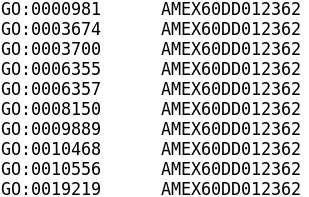
\includegraphics{images/axolotl-term2gene.png}
\caption{t2gene}
\end{figure}

\textbf{Example TERM2NAME format:}

\begin{figure}
\centering
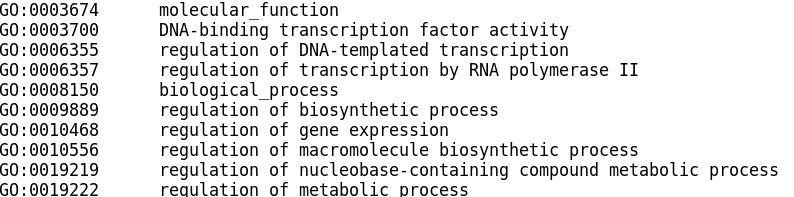
\includegraphics{images/axolotl-term2name.png}
\caption{t2name}
\end{figure}

There are then provided to the universal enrichment functions \texttt{GSEA} and \texttt{enricher} (ORA). It is essential that the gene lists provided have the same gene IDs as those in the \texttt{TERM2GENE} file.

In RStudio, we will extract these file formats from the eggNOG annotations file for axolotl and proceed with FEA.

Acknowledgement to \href{https://github.com/dadrasarmin}{Armin Dadras} for sharing his \href{https://github.com/dadrasarmin/enrichment_analysis_for_non_model_organism\%5D}{code} to extract \texttt{TERM2GENE} and \texttt{TERM2NAME} from \texttt{emapper} output.

\hypertarget{webgestaltr-1}{%
\subsection{WebGestaltR}\label{webgestaltr-1}}

This tool can perform ORA or GSEA for any organism with the provision of custom \texttt{GMT} and \texttt{description} file.

The \texttt{GMT} file format is slightly different than the typical \texttt{gene\ set\ matrix\ transposed\ file\ format} you may have seen before. For \texttt{WebGestaltR}, the tab-delimited GMT file with \texttt{.gmt} suffix has these columns:

\begin{enumerate}
\def\labelenumi{\arabic{enumi}.}
\tightlist
\item
  Gene set ID
\item
  Web link for gene set
\item
  Third and sunsequent columns are genes belonging to the gene set
\end{enumerate}

A typical \texttt{GMT} file has the gene set description in the second column. For \texttt{WebGestaltR}, the tab delimited \texttt{description} file with \texttt{.des} suffix has these columns:

\begin{enumerate}
\def\labelenumi{\arabic{enumi}.}
\tightlist
\item
  Gene set ID
\item
  Gene set description
\end{enumerate}

\begin{itemize}
\tightlist
\item
  \textbf{TBA:} - webgr file format images
\end{itemize}

\textbf{Example .gmt format:}

\begin{figure}
\centering
\includegraphics{images/webgr-gmt.png}
\caption{webgr-gmt}
\end{figure}

\textbf{Example TERM2NAME format:}

\begin{figure}
\centering
\includegraphics{images/webgr-des.png}
\caption{webgr-des}
\end{figure}

These files are then provided to the single FEA function within the package. The function has the same name as the package, \texttt{WebGestaltR}, with the parameter \texttt{enrichMethod} controlling whether ORA, GSEA or NTA is performed.

The \texttt{.gmt} file is provided to the parameter \texttt{enrichDatabaseFile} and the \texttt{.des} file is provided to the parameter \texttt{enrichDatabaseDescriptionFile}. Specifying \texttt{organism\ =\ "others"} is also required to run the FEA analysis with the custom databse files. Same as with \texttt{clsuterProfiler}, it is essential that the \texttt{.gmt} file has the same gene IDs as those in query gene list.

\begin{figure}
\centering
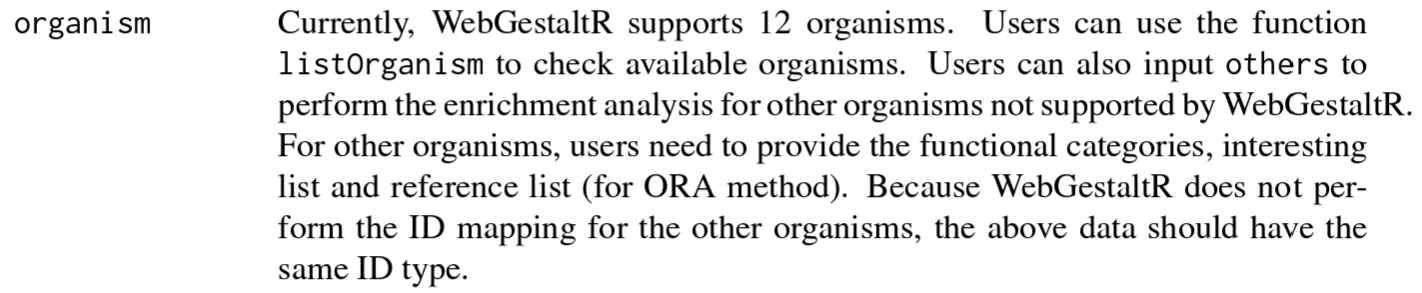
\includegraphics{images/webgestaltr-others-organisms.png}
\caption{webgr-others}
\end{figure}

\hypertarget{rnotebook-fea}{%
\section{RNotebook FEA}\label{rnotebook-fea}}

➤ Return to RStudio and open the notebook \texttt{novel\_species.Rmd}.

We will now continue with the activity in RStudio, before returning here to finish up with STRING web-based analysis.

\hypertarget{string-fea}{%
\section{STRING FEA}\label{string-fea}}

The axolotl putative proteome was previosuly uploaded to STRING and custom annotation performed. This completed using the STRING servers, with compute time less than one day.

~

Using the STRING web tool, we will now peform ORA of this custom axolotl annotation. We will not perform GSEA on STRING purely in the interest of time, as the processing takes a lot longer than ORA, however if you wish to run this at a late date, please go ahead!

➤ Open the following link in your browser:

\url{https://version-12-0.string-db.org/organism/STRG0A90SNX}

This will take you to the axolotl annotation page, where you can click \texttt{SELECT\ SPECIES\ ON\ INPUT\ PAGE} to add the custom species to the \texttt{Organisms} field, then toggle to your desired search type.

There is also a downloads page, where any of the STRING annotation files can be downloaded. If you wanted to use the STRING annotation files in \texttt{clusterProfiler} or \texttt{WebGestaltR}, you would download the \href{https://stringdb-downloads.org/download_proteomes/protein.enrichment.terms.v12.0/STRG0A90SNX.protein.enrichment.terms.v12.0.txt.gz}{`protein enrichment terms'} file and then extract the terms and axolotl gene IDs into the required formats, as we did for the eggNOG emapper annotations.

\begin{figure}
\centering
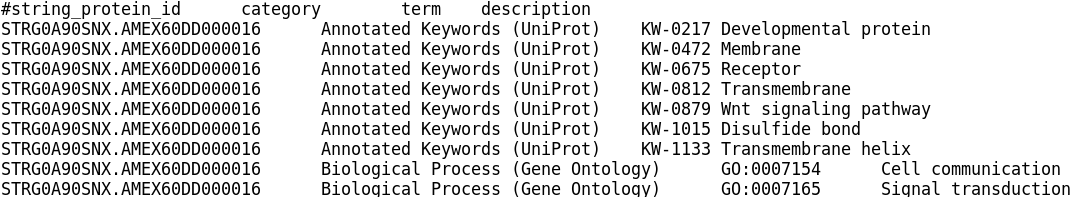
\includegraphics{images/string-enrichment-file-format.png}
\caption{string anno file format}
\end{figure}

➤ On STRING, click \texttt{SELECT\ SPECIES\ ON\ INPUT\ PAGE}, then from the left search options, select \texttt{Multiple\ proteins}.

Note that the \texttt{Organism} field is pre-filled with \texttt{STRG0A90SNX\ (axolotl)}.

➤ In the RStudio \texttt{Files} pane, locate your saved ORA gene list from earlier - \texttt{axolotl\_DEGs.txt}. Clcik the file to view it in RStudio, then copy the list into the STRING \texttt{List\ of\ Names} search field, then select \texttt{SEACRH}.

Click \texttt{CONTINUE} at the gene ID review page, and then explore the results!

Clicking on the \texttt{Analysis} tab will show the enichment tables with results for GO, STRING, KEGG, Reactome, TISSUES and UniProt.

Below the tables, under \texttt{Functional\ enrichment\ visualization} you can change \texttt{Category} to alter which databases results are plotted.

\hypertarget{how-do-the-string-results-compare-to-those-we-generated-in-r}{%
\subsection{How do the STRING results compare to those we generated in R?}\label{how-do-the-string-results-compare-to-those-we-generated-in-r}}

\begin{itemize}
\tightlist
\item
  \textbf{TBA:} - side by side plot comparison for STRING v R one of the ORA (CP GO, CO KEGG, WGR GO, or WGR KEGG)
\end{itemize}

We expect quite a bit of difference in the results because of the vast difference in annotation method.

\texttt{eggNOG\ emapper} appears more stringent than STRING in its similarity matches between the axolotl putative proteins and annotated orthologs. The table below compares the number of annotations yielded from the 47,196 putative axolotl proteins from both tools.

\begin{longtable}[]{@{}llll@{}}
\toprule\noalign{}
Method & GO & KEGG Pathways & All \\
\midrule\noalign{}
\endhead
\bottomrule\noalign{}
\endlastfoot
emapper & 21,376 & 12,229 & 39,539 \\
STRING & 36,895 & 21,502 & 38,398 \\
\end{longtable}

This suggests that the \texttt{emapper} results may be more specific, while the \texttt{STRING} results may be more sensitive. Using both methods for your novel speciues analysis may help validate and focus your FEA findings.

  \bibliography{book.bib,packages.bib}

\end{document}
